\documentclass[a4paper,11pt]{book}
\usepackage{chngpage}
%\documentclass[a4paper,twoside,11pt,titlepage]{book}
\usepackage{listings}
\usepackage{amssymb}
\usepackage{amsmath}
\usepackage{amsthm}
\usepackage[utf8]{inputenc}
\usepackage[spanish]{babel}
\usepackage{array}
\usepackage{url}
\usepackage{graphicx}
\usepackage{subfig}
% \usepackage[style=list, number=none]{glossary} %
%\usepackage{titlesec}
%\usepackage{pailatino}

\decimalpoint
\usepackage{dcolumn}
\newcolumntype{.}{D{.}{\esperiod}{-1}}
\makeatletter
\addto\shorthandsspanish{\let\esperiod\es@period@code}
\makeatother


\usepackage[chapter]{algorithm}
\RequirePackage{verbatim}
%\RequirePackage[Glenn]{fncychap}
\usepackage{fancyhdr}
\usepackage{graphicx}
\usepackage{afterpage}

\usepackage{longtable}

\usepackage[pdfborder={000}]{hyperref} %referencia

\tolerance=1
\emergencystretch=\maxdimen
\hyphenpenalty=10000
\hbadness=10000

% ********************************************************************
% Re-usable information
% ********************************************************************
\newcommand{\myTitle}{Criptosistemas en aplicaciones de mensajería\xspace}
\newcommand{\myDegree}{Doble grado en Ingeniería Informática y Matemáticas\xspace}
\newcommand{\myName}{Luis Tormo Fabios\xspace}
\newcommand{\myProf}{Pedro A. García Sánchez\xspace}
%\newcommand{\myOtherProf}{Nombre Apllido1 Apellido2 (tutor2)\xspace}
%\newcommand{\mySupervisor}{Put name here\xspace}
\newcommand{\myFaculty}{Escuela Técnica Superior de Ingenierías Informática y de
Telecomunicación\xspace}
\newcommand{\myFacultyShort}{E.T.S. de Ingenierías Informática y de
Telecomunicación y Facultad de Ciencias\xspace}
\newcommand{\myDepartment}{Departamento de ...\xspace}
\newcommand{\myUni}{\protect{Universidad de Granada}\xspace}
\newcommand{\myLocation}{Granada\xspace}
\newcommand{\myTime}{\today\xspace}
\newcommand{\myVersion}{Version 0.1\xspace}


\hypersetup{
pdfauthor = {\myName (email (en) ugr ()},
pdftitle = {\myTitle},
pdfsubject = {},
pdfkeywords = {palabra_clave1, palabra_clave2, palabra_clave3, ...},
pdfcreator = {LaTeX con el paquete ....},
pdfproducer = {pdflatex}
}

%\hyphenation{}


%\usepackage{doxygen/doxygen}
%\usepackage{pdfpages}
\usepackage{url}
\usepackage{colortbl,longtable}
\usepackage[stable]{footmisc}
%\usepackage{index}

%\makeindex
%\usepackage[style=long, cols=2,border=plain,toc=true,number=none]{glossary}
% \makeglossary

% Definición de comandos que me son tiles:
%\renewcommand{\indexname}{Índice alfabético}
%\renewcommand{\glossaryname}{Glosario}

\pagestyle{fancy}
\fancyhf{}
\fancyhead[LO]{\leftmark}
\fancyhead[RE]{\rightmark}
\fancyhead[RO,LE]{\textbf{\thepage}}
\renewcommand{\chaptermark}[1]{\markboth{\textbf{#1}}{}}
\renewcommand{\sectionmark}[1]{\markright{\textbf{\thesection. #1}}}

\setlength{\headheight}{1.5\headheight}

\newcommand{\HRule}{\rule{\linewidth}{0.5mm}}
%Definimos los tipos teorema, ejemplo y definición podremos usar estos tipos
%simplemente poniendo \begin{teorema} \end{teorema} ...
\newtheorem{teorema}{Teorema}[chapter]
\newtheorem{proposicion}[teorema]{Proposición}
\newtheorem{lema}[teorema]{Lema}
\newtheorem{ejemplo}[teorema]{Ejemplo}
\newtheorem{definicion}[teorema]{Definición}
\newtheorem{corolario}[teorema]{Corolario}
%\newenvironment{proof}{\paragraph{\emph{\textbf{Demostración.}}\\}}

\definecolor{gray97}{gray}{.97}
\definecolor{gray75}{gray}{.75}
\definecolor{gray45}{gray}{.45}
\definecolor{gray30}{gray}{.94}

\lstset{ frame=Ltb,
     framerule=0.5pt,
     aboveskip=0.5cm,
     framextopmargin=3pt,
     framexbottommargin=3pt,
     framexleftmargin=0.1cm,
     framesep=0pt,
     rulesep=.4pt,
     backgroundcolor=\color{gray97},
     rulesepcolor=\color{black},
     %
     stringstyle=\ttfamily,
     showstringspaces = false,
     basicstyle=\scriptsize\ttfamily,
     commentstyle=\color{gray45},
     keywordstyle=\bfseries,
     %
     numbers=left,
     numbersep=6pt,
     numberstyle=\tiny,
     numberfirstline = false,
     breaklines=true,
   }
 
% minimizar fragmentado de listados
\lstnewenvironment{listing}[1][]
   {\lstset{#1}\pagebreak[0]}{\pagebreak[0]}

\lstdefinestyle{CodigoC}
   {
	basicstyle=\scriptsize,
	frame=single,
	language=C,
	numbers=left
   }
\lstdefinestyle{CodigoC++}
   {
	basicstyle=\small,
	frame=single,
	backgroundcolor=\color{gray30},
	language=C++,
	numbers=left
   }

 
\lstdefinestyle{Consola}
   {basicstyle=\scriptsize\bf\ttfamily,
    backgroundcolor=\color{gray30},
    frame=single,
    numbers=none
   }


\newcommand{\bigrule}{\titlerule[0.5mm]}


%Para conseguir que en las páginas en blanco no ponga cabecerass
\makeatletter
\def\clearpage{%
  \ifvmode
    \ifnum \@dbltopnum =\m@ne
      \ifdim \pagetotal <\topskip
        \hbox{}
      \fi
    \fi
  \fi
  \newpage
  \thispagestyle{empty}
  \write\m@ne{}
  \vbox{}
  \penalty -\@Mi
}
\makeatother

\usepackage{pdfpages}
\begin{document}
\begin{titlepage}
 
 
\setlength{\centeroffset}{-0.5\oddsidemargin}
\addtolength{\centeroffset}{0.5\evensidemargin}
\thispagestyle{empty}

\noindent\hspace*{\centeroffset}\begin{minipage}{\textwidth}

\centering

 \vspace{3.3cm}


\includegraphics{imagenes/logo.png} 
 \vspace{0.5cm}

% Title

{\Huge\bfseries Criptosistemas en aplicaciones de mensajería\\
}
\noindent\rule[-1ex]{\textwidth}{3pt}\\[3.5ex]
{\large\bfseries Trabajo de fin de grado en Ingeniería Informática y Matemáticas\\[4cm]}
\end{minipage}

\vspace{2.5cm}
\noindent\hspace*{\centeroffset}\begin{minipage}{\textwidth}
\centering

\textbf{Autor}\\ {Luis Tormo Fabios}\\[2.5ex]
\textbf{Director}\\
Pedro A. García Sánchez\\
\textsc{---}\\
Granada, 7 de Septiembre de 2023
\end{minipage}

\vspace{\stretch{2}}

 
\end{titlepage}



%\chapter*{}
%\thispagestyle{empty}
%\cleardoublepage

%\thispagestyle{empty}

%\begin{titlepage}
 
 
\setlength{\centeroffset}{-0.5\oddsidemargin}
\addtolength{\centeroffset}{0.5\evensidemargin}
\thispagestyle{empty}

\noindent\hspace*{\centeroffset}\begin{minipage}{\textwidth}

\centering

 \vspace{3.3cm}


\includegraphics{imagenes/logo.png} 
 \vspace{0.5cm}

% Title

{\Huge\bfseries Criptosistemas en aplicaciones de mensajería\\
}
\noindent\rule[-1ex]{\textwidth}{3pt}\\[3.5ex]
{\large\bfseries Trabajo de fin de grado en Ingeniería Informática y Matemáticas\\[4cm]}
\end{minipage}

\vspace{2.5cm}
\noindent\hspace*{\centeroffset}\begin{minipage}{\textwidth}
\centering

\textbf{Autor}\\ {Luis Tormo Fabios}\\[2.5ex]
\textbf{Director}\\
Pedro A. García Sánchez\\
\textsc{---}\\
Granada, 7 de Septiembre de 2023
\end{minipage}

\vspace{\stretch{2}}

 
\end{titlepage}






%\cleardoublepage
%\thispagestyle{empty}

\begin{center}
{\large\bfseries Criptosistemas en aplicaciones de mensajería}\\
\end{center}
\begin{center}
Luis Tormo Fabios\\
\end{center}

%\vspace{0.7cm}
\noindent{\textbf{Palabras clave}: Criptografía simétrica, criptografía asimétrica, cuerpos finitos, intercambio de claves, curvas elípticas, funciones hash, protocolo criptográfico.}\\

\vspace{0.7cm}
\noindent{\textbf{Resumen}}\\

En esta memoria se realiza una descripción de los criptosistemas que utilizan las aplicaciones de mensajería instantáneas más populares. Para ello empiezo con un capítulo que introduce la criptografía simétrica y asimétrica. A continuación recuerdo algunos conceptos y resultados de la teoría de aritmética modular y cuerpos finitos necesaria para entender el funcionamiento de las distintas operaciones que se realizan en los distintos criptosistemas. Después describo el funcionamiento del criptosistema simétrico \emph{AES} y posteriormente describo los criptosistemas asimétricos usados, en este caso \emph{RSA} y el intercambio de claves \emph{Diffie-Hellman}. Como este tiene una versión usando Curvas Elípticas, también introduzco la teoría necesaria acerca de estas para describir su funcionamiento. Además, también dedico un capítulo a describir las funciones hash o resumen más usadas en los distintos criptosistemas. Para concluir explico el proceso criptográfico que siguen las aplicaciones de mensajería más populares e implemento una aplicación que implementa los criptosistemas más utilizados.

\cleardoublepage


\thispagestyle{empty}


\begin{center}
{\large\bfseries Cryptography in messaging app}\\
\end{center}
\begin{center}
Luis Tormo Fabios\\
\end{center}

%\vspace{0.7cm}
\noindent{\textbf{Keywords}: Symmetric cryptography, asymmetric cryptography, finite fields, key exchange, elliptic curves, hash functions, cryptographic protocol.}\\

\vspace{0.7cm}
\noindent{\textbf{Abstract}}\\

We live in an era in which social relationships cannot be conceived without thinking about social networks and in particular messaging applications. They allow us to connect, independently of physical barriers.

In this memory, the problem that I have approached has been the development of a theoretical study of the cryptosystems used by the most used messaging applications nowadays. For this purpose, I have developed in a rigorous way the mathematical and computational tools used by messaging applications. This development includes an introductory chapter in which I make an introduction to cryptography where I explain which are the objectives that cryptosystems have to fulfill to be valid and the attacks that they may be susceptible to, following the Kerchoffs principle. Then I explain the use of symmetric and asymmetric cryptosystems in instant messaging applications and I develop more extensively what symmetric cryptosystems are as well as the \emph{ECB}, \emph{CBC}, \emph{CFB} and \emph{GCM} modes of use. Finishing with an extensive development of what are the asymmetric cryptosystems.

In the next chapter, I recall some findings of modular arithmetic and finite fields necessary to understand the operation of cryptosystems such as \emph{AES} and \emph{RSA}. About modular arithmetic I develop some findings such as what is a congruence class, what are the arithmetic functions, the Chinese Remainder Theorem, findings of Euler's Phi function in particular, Euler's Theorem, and Fermat's Small Theorem among others.
On finite fields, I focus on the Galois field and the findings of this one that allows us to work with this one in a way that at a computational level to operate with this one is not so expensive than working with other fields allowing us to reduce in a significant way the computation time and the resources used.

Once the computer and mathematical tools have been introduced, I begin to explain the most widely used cryptosystems, starting with \emph{AES}.
In this chapter, I explain how \emph{AES} works. To do this I briefly introduce its history and develop its structure explaining the rounds that it performs explaining the operations that are carried out in each of them. These operations are \emph{ByteSub}, \emph{ShiftRows}, \emph{MixColumns} and \emph{AddRoundKey}. I finished the chapter explaining how the subkeys are calculated.

In the next chapter, I explain two fundamental asymmetric cryptosystems. These are \emph{RSA} and the \emph{Diffie-Hellman} key exchange protocol.
For \emph{RSA} I give a brief historical introduction and then I explain its procedures. Finally, I explain the digital signature using \emph{RSA}, a tool widely used for message validation.
For the \emph{Diffie-Hellman} key exchange I introduce \emph{The Discrete Logarithm Problem}, a problem through which the reliability of the \emph{Diffie-Hellman} key exchange is obtained. Once I saw this I explained the key exchange. Since there is a counterpart of this key exchange using \emph{Elliptic Curves} I introduce next all the theory of elliptic curves necessary to understand its operation. Once the theory is introduced I explain the \emph{Discrete Logarithm Problem} and the operation of the \emph{Diffie-Hellman} key exchange using \emph{Elliptic Curves}.

Having seen the main symmetric and asymmetric cryptosystems used by messaging applications, I have focused on explaining \emph{hash functions}.
To do this I have introduced what hash functions are and how they are constructed using the Merkle-Damgård Construction. This is a method that allows to construction of collision-resistant hash functions. Once I have seen how to build them I have described the operation of hash functions used in messaging applications. These are \emph{SHA-0}, \emph{SHA-1} and \emph{SHA-256}.

This part concludes the explanation of the computer and mathematical tools used by messaging applications and I have proceeded to explain the protocols used by the most widely used messaging applications today. 
The first protocol I developed was the \emph{MTProto protocol}, a protocol used by the Telegram messaging application. 
The next protocol I developed was \emph{the TextSecure Protocol}. Protocol used by WhatsApp, Facebook Messenger, and Signal applications among others.
Following this I have developed the protocol used by iMessage.
The last protocol I explained was \emph{Letter Sealing} used by the Line Messenger application.

Having seen this I have documented how I have developed a simple messaging application using the tools seen throughout the document. For this, I have used the \emph{Python} programming language. For this, I have used the Python programming language due to the amount of libraries it has making the work much easier. As task manager, I used \emph{PoeThePoet}, as dependency manager I used \emph{Poetry}, and as Test Runner I used \emph{Pytest}.
To create the interface I used \emph{Tkinter}, to establish the connections between devices I used the \emph{socket library}, and to create the cryptographic functions to encrypt the messages I used the \emph{Crypto library}.

Finally, I have concluded the paper with the conclusions and possible future work that I have been drawing during the development of this paper. I have also emphasized the emergence of post-quantum cryptography since in future times it will be necessary to protect our privacy since many of the current cryptosystems are vulnerable to attacks using quantum algorithms.
\chapter*{}
\thispagestyle{empty}

\noindent\rule[-1ex]{\textwidth}{2pt}\\[4.5ex]

Yo, \textbf{Luis Tormo Fabios}, alumno del doble grado de Ingeniería Informática y Matemáticas de la \textbf{Escuela Técnica Superior
de Ingenierías Informática y de Telecomunicación y la facultad de Ciencias de la Universidad de Granada}, con DNI 80169633M, autorizo la
ubicación de la siguiente copia de mi Trabajo Fin de Grado en la biblioteca del centro para que pueda ser
consultada por las personas que lo deseen.

\vspace{6cm}

\noindent Fdo: Luis Tormo Fabios

\vspace{2cm}

\begin{flushright}
Granada a 7 de Septiembre de 2023.
\end{flushright}


\chapter*{}
\thispagestyle{empty}

\noindent\rule[-1ex]{\textwidth}{2pt}\\[4.5ex]

D. \textbf{Pedro A. Garcı́a Sánchez}, Profesor del Área de Álgebra del Departamento Álgebra de la Universidad de Granada.

\vspace{0.5cm}

\textbf{Informan:}

\vspace{0.5cm}

Que el presente trabajo, titulado \textit{\textbf{Criptosistemas en aplicaciones de mensajería}},
ha sido realizado bajo su supervisión por \textbf{Luis Tormo Fabios}, y autorizamos la defensa de dicho trabajo ante el tribunal
que corresponda.

\vspace{0.5cm}

Y para que conste, expiden y firman el presente informe en Granada a 7 de Septiembre de 2023.

\vspace{1cm}

\textbf{El director:}

\vspace{5cm}

\noindent \textbf{Pedro A. Garcı́a Sánchez}

\chapter*{Agradecimientos}
\thispagestyle{empty}

       \vspace{1cm}


En primer lugar me gustaría agredecer a mi tutor del proyecto D. Pedro por su paciencia a la hora de corregir y su ayuda constante a la hora de resolver las distintas dudas y problemas que me han ido surgiendo a lo largo del desarrollo de este trabajo.\\
A todos los profesores que me han dado clase, en especial a las señoritas Isabel y Cati, Paco, Madre Andrea y D. Francisco Rojas, por confiar y enseñarme tanto.\\
A mi familia por estar presente a lo largo de estos años y en especial a mi madrina Tere y mi prima Mirian por animarme a cursar esta carrera.\\
A mi amigo Santi, porque a pesar de que dejó de estar con nosotros, nunca se fue del todo.\\
A mis abuelos, en especial a mi abuelo Juan, ya que creo que es la única persona con más ganas que yo de que termine.\\
A mis amigos, tanto a los de siempre por estar ahí todos estos años apoyándome, como  a los nuevos que me ha dado la carrera, por ser mis compañeros de fatiga. Gracias a vosotros esto ha sido mucho más fácil de llevar.\\
A Dani, Félix y Joaquín, por estar en las buenas y en las malas. Espero en los años futuros poder devolveros todo lo bueno que me habéis dado. Y si no, al menos la mitad.\\
A mis hermanos por ser uno de los motivos por los que me levanto todos los días.\\
Y por último a mis padres, por apostar por mí cuando nadie más lo hacía y no tirar la toalla, ver en mi un potencial que no sabía que tenía y aguantarme cuando no fue fácil. Si no fuera por vosotros, esto no habría sido posible.


\frontmatter
\tableofcontents
%\listoffigures
%\listoftables
%
\mainmatter
\setlength{\parskip}{5pt}

\chapter{Introducción}
Vivimos en una época en la que no se pueden concebir las relaciones sociales sin pensar en las redes sociales y en particular las aplicaciones de mensajería. Estas nos permiten conectarnos unos con otros independientemente de las barreras físicas.
Hay aplicaciones como  \emph{WhatsApp}, \emph{Facebook Messenger} o \emph{Telegram} que tienen 2.000, 931 y 700 millones de usuarios respectivamente, lo que supone un porcentaje significativo de la población mundial que usa aplicaciones de mensajería.\\  
Debido a esta enorme cantidad de usuarios las aplicaciones tienen que garantizar su seguridad y la privacidad. Es por esto que la criptografía ha cobrado un papel fundamental en la actualidad ya que las herramientas que ofrece son las que permiten garantizar dicha seguridad y privacidad de los usuarios de las aplicaciones. 

\section{Contexto histórico}
Las aplicaciones de mensajería aparecieron en la década de 1970. Una de las primeras fue el sistema \emph{PLATO}, este era una aplicación de asistencia para la computadora basada en un sistema informático de tiempo compartido por usuarios y programadores. Fue diseñada por Bitzer con la finalidad de hacer realidad el objetivo de educar por el ordenador y entre una de sus funcionalidades había un chat para que los usuarios se comunicaran entre sí de manera local.\\ 
Entre las décadas de 1980 y 1990 apareció la aplicación \emph{TALK}, esta fue diseñada para dispositivos con sistema operativos basados en \emph{UNIX/LINUX}. Esta aplicación permitía enviar mensajes entre usuarios a través de Internet. Si bien al principio solo permitía comunicarse entre usuarios que estuvieran conectados al mismo dispositivo aunque luego se amplió la funcionalidad permitiendo el envío de mensajes entre usuarios de otros sistemas.\\
Hasta 1996 no apareció una aplicación de mensajería que se pudiera usar en otros dispositivos con distintos sistemas operativos. 
Esta fue \emph{ICQ} y supuso un antes y un después ya que fue la primera en abarcar tantos usuarios y además añadió nuevas funcionalidades. En su momento de mayor popularidad alcanzó los 38 millones de usuarios, permitiendo atisbar el potencial de las aplicaciones de mensajería como medio de comunicación.
Esta aplicación añadía nuevas funcionalidades como eran un perfil de usuario personalizable, estado de conexión, emoticonos, transferencia de contactos, transferencia de archivos y chat grupales que fueron adoptadas por las nuevas aplicaciones de mensajería manteniéndose muchas de ellas hasta hoy en día.\\
A partir de esta empezaron a surgir nuevas aplicaciones de mensajería con mayor frecuencia, estas aplicaciones usaban cada una un protocolo distinto por lo que se llevó a los usuarios a tener distintos clientes para cada aplicación.
Algunas de las aplicaciones más populares que aparecieron en esta época fueron \emph{MSN Messenger} y \emph{AIM}. La más popular fue \emph{AIM} que en 2006 tenía el control del 52 por ciento del mercado de las aplicaciones de mensajería. \emph{MSN} necesito más años para ser más popular y hasta 2005 que no alcanzó su mayor pico llegando a atraer alrededor de 330 millones de usuarios activos cada mes. Lo hizo bajo el nombre de \emph{Windows Live Messenger}.\\ 
Para compensar el creciente número de protocolo surgieron aplicaciones multiclientes que permitían soportar varios de estos protocolos, algunas de estas fueron \emph{Pidgin} o \emph{Trillian}. Ambas aplicaciones permitían comunicarse usando protocolos como \emph{MSN}, \emph{MySpaceIM}, \emph{XMPP/Jabber(Google Talk, Facebook Messenger)} y \emph{Yahoo!} entre otros.\\ 
A la vez se popularizaron las videollamadas por lo que aparecieron nuevas aplicaciones para aprovechar el nuevo nicho. Una de las primeras en aparecer fue \emph{Microsoft NetMeeting} aunque poco después apareció \emph{Skype} y se apropió de la mayoría de los usuarios de esta.\\
En 2010 los desarrolladores cambiaron de plataforma y dejaron de desarrollar aplicaciones de mensajería para ordenador para centrarse en los \emph{Smartphones}. Aparecieron aplicaciones como \emph{WhatsApp, Telegram} y \emph{Facebook Messenger} que como hemos visto al principio del capítulo, son fundamentales hoy en día y abarcan miles de millones de usuarios.

\section{Descripción del problema}
En esta memoria el problema que he abordado ha sido el desarrollo de un estudio teórico de los criptosistemas que utilizan las aplicaciones de mensajería más utilizadas en la actualidad. Para ello se desarrolla de manera rigurosa de las herramientas matemáticas e informáticas que utilizan estas. Este desarrollo abarca una introducción a la criptografía simétrica y asimétrica así como teoría de cuerpos finitos necesarios para entender adecuadamente las herramientas.
Un desarrollo en profundidad de los cifrados de bloque y del cifrado \emph{AES} en particular explicación exhaustiva de \emph{RSA} y del \emph{Problema del Logaritmo discreto} y como resultado de este, el intercambio de claves \emph{Diffie-Hellman}. Posteriormente he introducido la teoría de Curvas Elípticas necesaria para entender el análogo de las herramientas anteriores utilizando este cuerpo.
Después he introducido las \emph{funciones hash}, como construirlas usando la construcción de \emph{Merkle-Damgård} y las familias de funciones más utilizadas en las aplicaciones de mensajería actuales. A continuación he realizado una descripción como incorporan las aplicaciones de mensajería más populares los criptosistemas vistos anteriormente. Por último he desarrollado una aplicación de mensajería en la cual he aplicado lo visto previamente en la memoria \emph{Desarrollar esto más extensamente cuando tenga la aplicación}. 

\section{Técnicas utilizadas}
Las herramientas matemáticas utilizadas han sido las siguientes.
\begin{itemize}
	\item Teoría de cuerpos
	\item Teoría de números
	\item Teoría de grupos
\end{itemize}

Y las herramientas informáticas
\begin{itemize}
	\item Criptografía
	\item Algorítmica
\end{itemize}

		

%
\chapter{Criptografía y Curvas Elípticas}
%\noindent\rule[-1ex]{\textwidth}{2pt}\\[4.5ex]

En este capítulo se introducirá la teoría sobre criptografía y curvas elípticas necesaria para entender la base detrás de los criptosistemas usados en las aplicaciones de mensajería más populares.

\section{Objetivos de la criptografía}
En este apartado voy a hablar sobre los objetivos de un criptosistema y los posibles ataques que se le pueden hacer, así como una introducción a la criptografía simétrica y asimétrica y su uso en las aplicaciones de mensajería que nos ayudará a entender los distintos criptosistemas de los que se hablará después.
Mayormente la información de este apartado ha sido obtenida de \cite{apuntesCriptografia} para los criptosistemas simétricos y \cite{angelRiosMateos} para los cifrados asimétricos.\\
Los principales objetivos que debe cumplir todos los criptosistemas son:
\begin{description}
	\item \textbf{Confidencialidad}\\ 
		La información solo puede ser accesible por las entidades autorizadas. 
	\item \textbf{Integridad}\\ 
		La información no ha sido alterada en el envío.
	\item \textbf{Autenticidad}\\ 
		La información proviene de quién afirma haberla enviado.
	\item \textbf{No repudio}\\ 
		El emisario de una información no puede a posteriori negar que se realizado tal envío.
\end{description}

Para hablar de los ataques supondremos que se sigue el principio de \emph{Kerckhoffs}, el cual establece que el adversario conoce todos los detalles del criptosistema excepto la clave empleada.\\
Los posibles ataques son:
\begin{description}
		\item \textbf{Criptograma}\\ El adversario conoce el criptograma, es decir, el mensaje cifrado o un fragmento de este.
		\item \textbf{Mensaje Conocido}\\ El atacante conoce parejas mensaje/criptograma cifradas con una misma clave.
		\item \textbf{Mensaje escogido}\\ El atacante puede generar criptogramas para mensajes de su elección. Una vez obtenidas dichas parejas, trata de averiguar el mensaje correspondiente a un criptograma desconocido.
		\item \textbf{Mensaje escogido-adaptativo}\\ El atacante no solo puede generar pareas mensaje/criptograma a su elección, sino que puede hacerlo tantas veces como quiera realizando los análisis que considere oportunos.
		\item \textbf{Criptograma escogido y escogido-adaptativo}\\ Similar a los anteriores pero partiendo del criptograma, teniendo acceso a descifrar los criptogramas que desee, inicialmente o a lo largo del proceso. Lo que se busca en este ataque es la clave.
\end{description}

Una vez vistos los objetivos que tienen que cumplir los criptosistemas y los posibles ataques veamos qué el uso de los criptosistemas simétricos y asimétricos en las aplicaciones de mensajería y posteriormente una introducción más técnica de estos.\\

\subsection{Criptosistemas simétricos y asimétricos en las aplicaciones de mensajería}
Los criptosistemas simétricos y asimétricos conforman una parte fundamental de las aplicaciones de mensajería, ambos son usados a la par de manera complementaria.\\
Los criptosistemas simétricos debido a su velocidad de cifrado, su uso reducido de recursos y su mejor manejo de grandes cantidades de datos se suelen utilizar para cifrar los mensajes. 
Pero como tienen el defecto de que si la clave es interceptada el criptosistema es vulnerado y se pierde tanto la confidencialidad como la autenticidad de los mensajes.\\ 
Para evitar esto se suele complementar con métodos seguros para el intercambio de la clave como puede ser el \emph{intercambio de claves Diffie-Hellman}.\\
Los cifrados asimétricos son muy utilizados para la firma y autentificación de los mensajes, garantizando de esta manera la seguridad de la aplicación y se complementan con cifrados simétricos a la hora de cifrar los mensajes para garantizar de esta forma una eficiencia mucho mayor. Ya que uno de los principales problemas que tienen es su complejidad algorítmica a la hora de cifrar y descifrar los mensajes.\\

\subsection{Criptosistema simétrico}
Un criptosistema simétrico es un criptosistema en el cual se utiliza una sola clave para cifrar y descifrar un mensaje. La importancia para garantizar la seguridad de los criptosistemas simétricos reside en el secreto de la clave mientras que el conocer el algoritmo utilizado no es tan importante como medida de seguridad. Es decir, lo importante es que el atacante no conozca la clave, mientras que conozca el algoritmo usado no lo es tanto.\\
Un criptosistema simétrico está formado por:
\begin{itemize}
	\item $\mathcal{M}$ el conjunto de los mensajes, elementos candidatos a ser encriptados.
	\item $\mathcal{C}$ el conjunto de los criptogramas o mensajes obtenido después del proceso de encriptar.
	\item $\mathcal{K} \subseteq \mathcal{K}_p\times\mathcal{K}_s$ el espacio de las claves, elementos que se utilizan para encriptar y desencriptar los mensajes. 
\end{itemize}
Un criptosistema simétrico viene definido por dos aplicaciones
$$E:\mathcal{K}_p\times\mathcal{M}\rightarrow\mathcal{C},$$
$$\mathcal{D}:\mathcal{K}_s\times\mathcal{C}\rightarrow\mathcal{M}.$$
tales que para cualquier clave $k_p \in \mathcal{K}_p$, existe una clave $k_s$ de manera que dato cualquier mensaje $m \in \mathcal{M}$,
$$
\mathcal{D}(k_s,E(k_p,m))=m.
$$
Fijada la clave $k_p \in \mathcal{K}_p$ y su correspondiente $k_s \in \mathcal{K}_s$ se definen las funciones de cifrado y descifrado como:\\
\begin{aligned}
	\center
	&$E_{k_p}:\mathcal{M}\rightarrow\mathcal{C},$\\
	&$E_{k_p}(m)=E(k_p,m),$
\end{aligned}
\begin{aligned}
	\center
	&$D_{k_p}:\mathcal{C}\rightarrow\mathcal{M},$\\
	&$D_{k_s}(c)=D(k_s,c).$
\end{aligned}

\subsection{Criptosistema asimétrico}
Un criptosistema asimétrico es un criptosistema en el cual se utilizan dos claves, una para cifrar el mensaje y otra para descifrarlo. La clave para cifrar es la que se conoce como \emph{clave pública}, mientras que la que se utiliza para descifrar es la \emph{clave privada}. Estos criptosistemas surgieron para paliar la debilidad de los criptosistemas simétricos, que es que la clave que cifra y descifra se tiene que compartir, pudiendo esta ser interceptada.  La seguridad de estos criptosistemas reside en que no se conozcla la clave privada.\\
Un criptosistema asimétrico está formado por:
\begin{itemize}
	\item $\mathcal{M}$ es el conjunto de los mensajes.
	\item $\mathcal{C}$ es el conjunto de los criptogramas.
	\item Una función $P:\mathcal{K}' \rightarrow \mathcal{K}$, que nos permitirá generar la clave pública.
\end{itemize}
Un criptosistema asimétrico viene definido por dos aplicaciones:
$$E:\mathcal{K}\times\mathcal{M}\rightarrow\mathcal{C},$$
$$\mathcal{D}:\mathcal{K}'\times\mathcal{C}\rightarrow\mathcal{M},$$
tales que para cualquier clave privada $k' \in \mathcal{K}'$ obtenemos la clave pública como $P(k')=k$ y se definen las funciones de cifrado y descifrado como:\\
\begin{aligned}
	\center
	&$E_{k}:\mathcal{M}\rightarrow\mathcal{C},$\\
	&$E_{k}(m)=E(k,m),$
\end{aligned}
\begin{aligned}
	\center
	&$D_{k^{'}}:\mathcal{C}\rightarrow\mathcal{M},$\\
	&$D_{k'}(c)=D(k',c).$
\end{aligned}

Para que un criptosistema asimétrico sea seguro tenemos que garantizar:
\begin{itemize}
	\item $P$ es una función de dirección única, es decir, que dado un elemento de su imagen no se puede calcular su imagen inversa fácilmente.
	\item Para la mayoría de los $k \in \mathcal{K}$, la aplicación $E_k$ es de dirección única.
	\item $\mathcal{D}_{k'}$ se puede calcular en un periodo corto de tiempo si se conoce $k'$ y que sea imposible o el periodo sea muy largo en caso de solo conocerse $k$.
\end{itemize}

\subsection{Cifrados de bloque}
A continuación se introducirá los cifrados de bloque, necesarios para entender el algoritmo \textbf{Rindael AES} que se explicará posteriormente. La información ha sido obtenida de \cite{apuntesCriptografia}.\\
Los cifrados de bloque son criptosistemas de clave simétrica en los que la longitud de los bloques y claves es fija.\\
Este criptosistema se define
$$
	E:\mathbb{B}^K\times\mathbb{B}^N\rightarrow \mathbb{B}^N,
$$
$$
	D:\mathbb{B}^K\times\mathbb{B}^N\rightarrow \mathbb{B}^N,
$$
Donde N es el tamaño del bloque y K es el tamaño de la clave.\\
Los cifrados tienen distintos modos de operación los cuales dependen solo del tamaño del bloque. Estos modos permiten garantizar la confidencialidad de los mensajes, si bien, no garantizan su integridad. La información para describir los modos la he complementado con \cite{bloquenuevo}.\\ 
Los distintos modos usados en los cifrados de bloque son:\\
\begin{itemize}
	\item \textbf{Electronic CodeBook}\\
	Modo en el cual para una clave dada, se le asigna un bloque de texto fijo cifrado por cada bloque de texto plano. Los pasos que se siguen para encriptar y desencriptar son:
	\begin{itemize}
		\item \textbf{\emph{Cifrado ECB}}
		\begin{description}
			\item Dividimos m en $m_{[1]}\dots m_{[l]}$ con $m_{[i]} \in \mathbb{B}^N$
			\item Para $i\in \{1,\dots,l\}$ hacer
			\begin{description}
				\item $c_{[i]} = E_k(m_{[i]})$
			\end{description}
			\item Devolvemos $c_{[1]}\dots c_{[l]}$
		\end{description}

		\item \textbf{\emph{Descifrado ECB}}
		\begin{description}
			\item Dividimos c en $c_{[1]}\dots c_{[l]}$ con $c_{[i]} \in \mathbb{B}^N$
			\item Para $i\in\{1,\dots,l\}$ hacer
			\begin{description}
				\item $m_{[i]} = D_k(c_{[i]})$
			\end{description}
			\item Devolvemos $m_{[1]}\dots m_{[l]}$
		\end{description}
	\end{itemize}
\newpage
		\begin{figure}[htb]
			\centering
			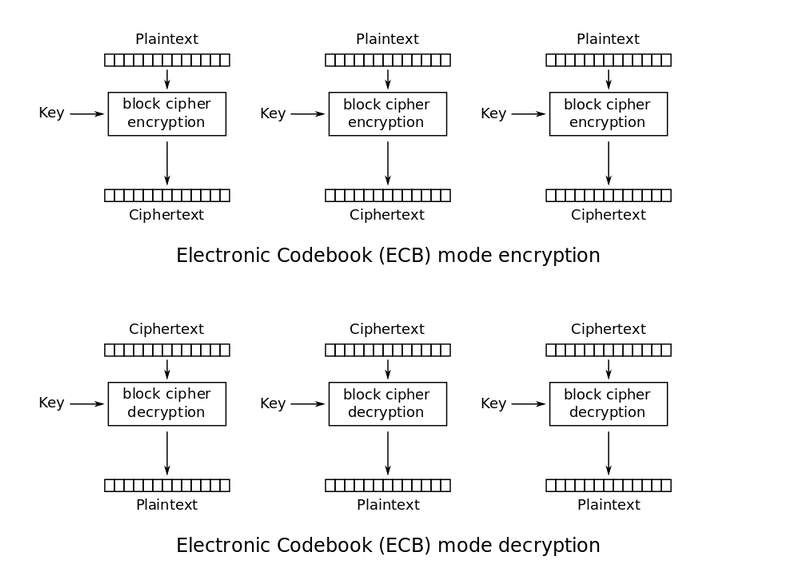
\includegraphics[scale=0.4]{imagenes/ecb.png} 
			\caption{Esquema del cifrado y descifrado del modo ECB \cite{cifradobloque}.}
			\label{esquemaecb}
		\end{figure}
		
	\item \textbf{Cipher-Block Chaining}\\
	En este modo se combina los bloques de texto plano con los bloques de texto cifrados anteriormente. Para cifrar el primer bloque será necesario un bloque inicial, $c_{[0]}$, el cual no tiene necesariamente que ser secreto. Los pasos seguidos para encriptar y desencriptar son:
	\begin{itemize}
		\item \textbf{\emph{Cifrado CBC}}
		\begin{description}
			\item $c_{[0]} \in \mathbb{B}^*$
			\item Dividimos m en $m_{[1]}\dots m_{[l]}$ con $m_{[i]} \in \mathbb{B}^N$
			\item Para $i\in\{1,\dots,l\}$ hacer
			\begin{description}
				\item $c_{[i]} = E_k(m_{[i]}\oplus c_{[i-1]})$
			\end{description}
			\item Devolvemos $c_{[1]}\dots c_{[l]}$
		\end{description}

		\item \textbf{\emph{Descifrado CBC}}
		\begin{description}
			\item Dividimos c en $c_{[0]}\dots c_{[l]}$ con $c_{[i]} \in \mathbb{B}^N$
			\item Para $i\in\{1,\dots,l\}$ hacer
			\begin{description}
				\item $m_{[i]} = D_k(c_{[i]})\oplus c_{[i]}$
			\end{description}
			\item Devolvemos $m_{[1]}\dots m_{[{l}]}$
		\end{description}
	\end{itemize}
\newpage
		\begin{figure}[htb]
			\centering
			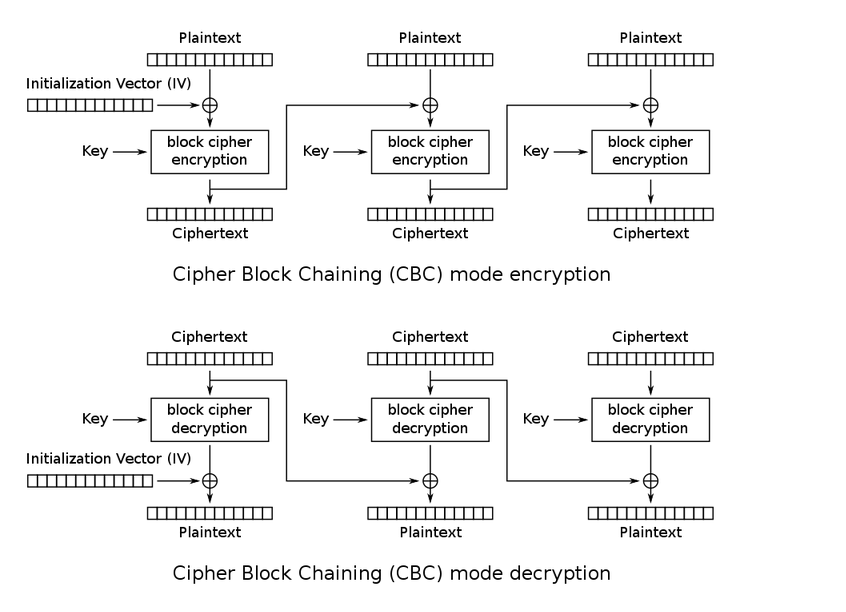
\includegraphics[scale=0.4]{imagenes/cbc.png} 
			\caption{Esquema del cifrado y descifrado del modo CBC \cite{cifradobloque}.}
			\label{esquemacbc}
		\end{figure}

	\item \textbf{Cipher FeedBack}\\
	Modo en el cual se combina cada bloque de texto plano del mensaje consigo mismo encriptado, los pasos que se siguen son:
	\begin{itemize}
		\item \textbf{\emph{Cifrado CFB}}
		\begin{description}
			\item $x_{[0]} \in \mathbb{B}^r$
			\item Dividimos m en $m_{[1]}\dots m_{[l]}$ con $m_{[i]} \in \mathbb{B}^N$
			\item Para $i\in\{1,\dots,l\}$ hacer
			\begin{description}
				\item $c_{[i]} = m_{[i]}\oplus msb_r(E_k(x_{[i]}))$
				\item $x_{[i+1]} = lsb_{N-r}(x_i)||c_{[i]$
			\end{description}
			\item Devolvemos $c_{[1]}\dots c_{[l]}$
		\end{description}

		\item \textbf{\emph{Descifrado CFB}}
		\begin{description}
			\item Dividimos c en $c_{[1]}\dots c_{[l]}$ con $c_{[i]} \in \mathbb{B}^r$
			\item Para $i\in\{1,\dots,l\}$ hacer
			\begin{description}
				\item $m_{[i]} = c_{[i]}\oplus msb_r(E_k(x_{[i]}))$
				\item $x_{[i+1]} = lsb_{N-r}(x_i)||c_{[i]$
			\end{description}
			\item Devolvemos $m_{[1]}\dots m_{[l]}$
		\end{description}
	\end{itemize}

%\newpage
		\begin{figure}[htb]
			\centering
			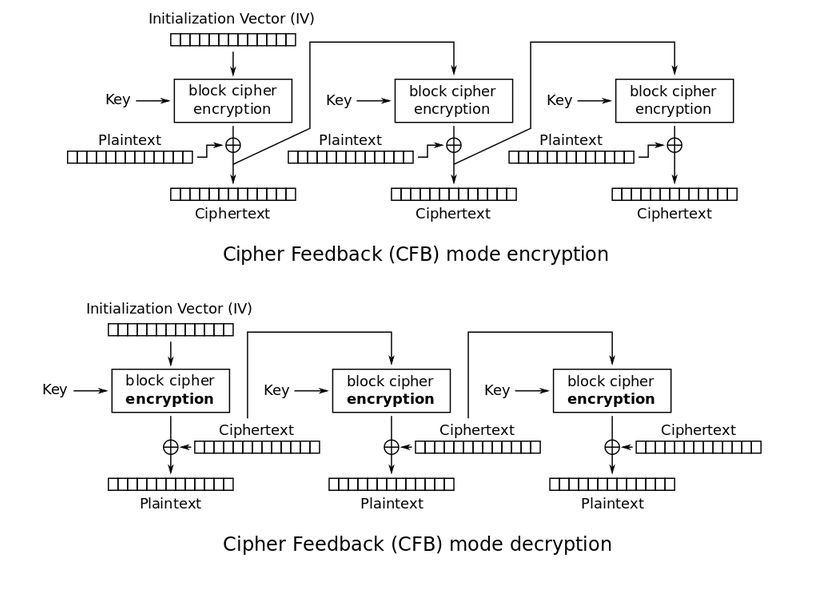
\includegraphics[scale=0.4]{imagenes/cfb.png} 
			\caption{Esquema del cifrado y descifrado del modo CFB \cite{cifradobloque}.}
			\label{esquemacfb}
		\end{figure}

\newpage
	\item \textbf{Output FeedBack}\\
	Modo en el cual se parte de un bloque inicial $x_{[0]}$ único y secreto. En cada iteración se encripta este y se combina con un bloque del mensaje sin cifrar de manera recursiva. Los pasos seguidos para encriptar y desencriptar son:
	\begin{itemize}
		\item \textbf{\emph{Cifrado OFB}}
		\begin{description}
			\item $x_{[0]} \in \mathbb{B}^N$
			\item Dividimos m en $m_{[1]}\dots m_{[l]}$ con $m_{[i]} \in \mathbb{B}^N$
			\item Para $i\in\{1,\dots,l\}$ hacer
			\begin{description}
				\item $x_{[i]} = E_k(x_{[i-1]})$
				\item $c_{[i]} = m_{[i]}\oplus x_{[i]}$
			\end{description}
			\item Devolvemos $c_{[1]}\dots c_{[l]}$
		\end{description}

%\newpage
		\item \textbf{\emph{Descifrado OFB}}
		\begin{description}
			\item Dividimos c en $c_{[1]}\dots c_{[l]}$ con $c_{[i]} \in \mathbb{B}^N$
			\item Para $i\in\{1,\dots,l\}$ hacer
			\begin{description}
				\item $x_{[i]} = E_k(x_{[i-1]})$
				\item $m_{[i]} = c_{[i]}\oplus x_{[i]}$
			\end{description}
			\item Devolvemos $m_{[1]}\dots m_{[l]}$
		\end{description}
	\end{itemize}
		\begin{figure}[htb]
			\centering
			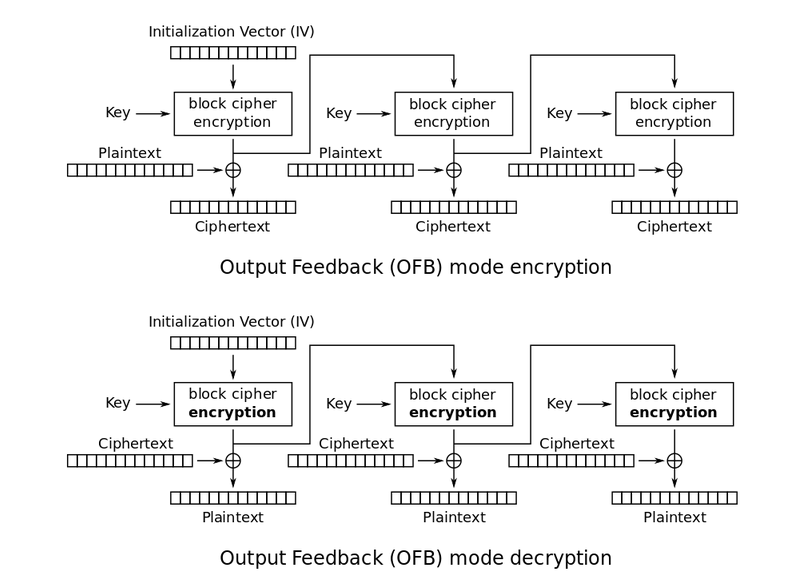
\includegraphics[scale=0.4]{imagenes/ofb.png} 
			\caption{Esquema del cifrado y descifrado del modo OFB \cite{cifradobloque}.}
			\label{esquemaofb}
		\end{figure}
\end{itemize}
\newpage
Como podemos ver, el más sencillo es ECB ya que lo único que hace es fragmentar el mensaje en bloques y encriptar individualmente cada bloque. En CBC, CFB y OFB se parte de un bloque inicial y se generan bloques nuevos de manera recursiva operando con ellos de manera disinta en fución de cada modo.\\ 
En CBC se realiza la operación $\oplus$ de cada bloque generado encriptandose el bloque cifrado previo a esta con un bloque del mensaje, los nuevos bloques son los resultados de la operación anterior.\\
En CFB se coge el bit menos significativo de resultado de encriptar el bloque generado previo y se hace la operación $\oplus$ con cada bloque del mensaje. Para generar un nuevo bloque se combina el mensaje cifrado previo con el bit menos significativo del conjunto de bits $N-r$ del bloque generado anterior con la operación $||$.\\
Y en OFB se realiza la operación $\oplus$ de el resultado de encriptar el bloque generado previo con un bloque del mensaje.\\
Actualmente el más utilizado en las aplicaciones de mensajería es el modo CBC. Esto es debido a que es relativamente fácil de implementar y además permite encriptar en paralelo.
\section{El algoritmo Rijndael AES}
En esta sección hablaré sobre el cifrado Rijndael AES el cual es un cifrado de bloque simétrico muy utilizado actualmente por aplicaciones como \emph{Telegram}, \emph{WhatsApp} y \emph{FacebookChat} entre otras.\\
El algoritmo Rijndael llamado así en honor a sus dos autores Joan Daemen y Vicent Rijmen, es un algoritmo de cifrado por bloques que fue adoptado en octubre de 2000 por el NIST (\emph{National Institute for Standards and Technology}) para su empleo en aplicaciones criptográficas no militares en sustitución del algoritmo \emph{DES} después de un proceso de más tres años en los que se buscaba un algoritmo que fuera potente, eficiente y fácil de implementar.\\
Está diseñado para manejar longitudes de clave y de bloque variables entre los 128 y los 256 bits y aunque estos sean variables, en el estándar adoptado por el Gobierno de Estados Unidos en 2001 \cite{aesUsa} establece una longitud fija de bloque de 128 bits y una longitud de clave a escoger entre 128, 192 y 256 bits.\\
La información para los siguientes apartados de AES la he obtenido de \cite{En2011}.\\

\subsection{Estructura de AES}
%\subsection{Elementos de AES}
AES es un algoritmo que se basa en aplicar un número determinado de rodas a un valor intermedio denominado \emph{estado} que puede ser representado por una matriz rectangular que posee cuatro filas y $N_{b}$ columnas. Análogamente la clave tiene la misma estructura, una matriz de cuatro filas y $N_{k}$.
El bloque a cifrar o descifrar se traslada directamente byte a byte sobre la matriz de estado de columna en columna($a_{0,0}, a_{1,0}, a_{2,0}, a_{3,0}, a_{0,1} ...$)

\begin{table}[htb]
	\begin{center}
		\begin{tabular}{| l | l | l | l |}
				\hline
				$\math{a}_{0,0}$ & $\math{a}_{0,1}$ & $\math{a}_{0,2}$ & $\math{a}_{0,3}$\\ \hline
				$\math{a}_{1,0}$ & $\math{a}_{1,1}$ & $\math{a}_{1,2}$ & $\math{a}_{1,3}$\\ \hline
				$\math{a}_{2,0}$ & $\math{a}_{2,1}$ & $\math{a}_{2,2}$ & $\math{a}_{2,3}$\\ \hline
				$\math{a}_{3,0}$ & $\math{a}_{3,1}$ & $\math{a}_{3,2}$ & $\math{a}_{3,3}$\\ \hline
		\end{tabular}
		\caption{Ejemplo de matriz de estado con $N_b=4$(128 bits).}
	\end{center}
\end{table}

\begin{table}[htb]
	\begin{center}
		\begin{tabular}{| l | l | l | l |}
				\hline
				$\math{k}_{0,0}$ & $\math{k}_{0,1}$ & $\math{k}_{0,2}$ & $\math{k}_{0,3}$\\ \hline
				$\math{k}_{1,0}$ & $\math{k}_{1,1}$ & $\math{k}_{1,2}$ & $\math{k}_{1,3}$\\ \hline
				$\math{k}_{2,0}$ & $\math{k}_{2,1}$ & $\math{k}_{2,2}$ & $\math{k}_{2,3}$\\ \hline
				$\math{k}_{3,0}$ & $\math{k}_{3,1}$ & $\math{k}_{3,2}$ & $\math{k}_{3,3}$\\ \hline
		\end{tabular}
		\caption{Ejemplo de clave con $N_k=4$(128 bits).}
	\end{center}
\end{table}

En otros casos el bloque y la clave pueden ser representados como vectores de registro de 32 bits donde cada registro esta compuesto por los bytes de la columna correspondiente ordenados en orden descendiente.\\

Siendo $B$ el bloque que queremos cifrar y $S$ la matriz de estado, el algoritmo AES con $n$ rondas quedaría:

\begin{enumerate}
	\item Calcular $K_0, K_1,...,K_n$ subclaves a partar de la clave $K$.
	\item $S\leftarrow B \oplus K_0$
	\item Para $i=1$ hasta $n$ hacer
	\begin{description}
			\item Aplicar la roda \emph{i}-ésima del algoritmo con la subclave $K_i$
	\end{description}
\end{enumerate}
Como las funciones usadas en cada ronda son invertibles, para descifrar aplicaremos las funciones inversas de las funciones usadas para cifrar en el orden opuesto.

\begin{table}[htb]
	\begin{center}
		\begin{tabular}{| l | l | l | l |}
				\hline
				& $N_b = 4$(128 bits) & $N_b = 6$(192 bits)& $N_b = 8$(256 bits)\\ \hline
				$N_k = 4$(128 bits)& 10 & 12 & 14\\ \hline
				$N_k = 6$(128 bits)& 12 & 12 & 14\\ \hline
				$N_k = 8$(128 bits)& 14 & 14 & 14\\ \hline
		\end{tabular}
		\caption{Número de rodas en función del tamaño de la clave y bloque}
		\label{rondas_aes}
	\end{center}
\end{table}


En el algoritmo AES se define cada ronda como una composición de cuatro funciones invertibles diferentes, formando tres \emph{capas}. Estas funciones tienen un propósito específico:
\begin{itemize}
	\item \textbf{Capa de mezcla lineal:} Formada por las funciones \emph{DesplazarFila} y \emph{MezclarColumnas} y permite obtener un alto nivel de difusión a lo largo de varias rondas.
	\item \textbf{Capa no lineal:} Formada por la función \emph{ByteSub} y es la aplicación paralela de s-cajas con propiedades óptimas de no linealidad.
	\item \textbf{Capa de adición de clave:} Es un simple \emph{or-exclusivo} entre el estado intermedio y la subclave correspondiente a cada ronda.
\end{itemize}

\subsection{El cuerpo de Galois $\operatorname{GF}(2^n)$}
Antes de desarrollar las rondas de AES y posteriormente la teoría de Curvas Elípticas en $\operatorname{GF}(2^n)$ introduciré el cuerpo $\operatorname{GF}(2^n)$ el cual tiene una serie de propiedades que lo hacen muy interesante y justifican su uso tan extendido en criptografía.\\
El conjunto $\mathbb{Z}_2[x]$ es el conjunto de polinomios con coeficientes en $\mathbb{Z}_2$ es decir, el el conjunto de polinomios cuyos coeficientes solo valen 0 o 1. Por lo que los polinomios pueden ser representados por una cadena de bits.
 Un ejemplo sería el polinomio $f(x)=x^4+x^3+x+1$ que quedaría representado como 11011. 
Además si lo sumamos con otro polinomio como puede ser $g(x)=x^2+x+1$ tenemos que $f(x)+g(x)=x^4+x^3+x^2$ que equivale a hacer la operación \emph{xor} entre 11011 y 00111, por lo que a nivel computacional, es muy fácil implementar estas operaciones.\\
Escogiendo un polinomio irreducible en $\mathbb{Z}_2$ podemos generar un cuerpo de Galois. Este conjunto es representado como $\operatorname{GF}(2^n)$, donde $n$ es el grado del polinomio irreducible que lo genera.\\
Las principales ventajas que tiene trabajar con $\operatorname{GF}(2^n)$ es que permite llevar a cabo implementaciones de una sencillez significativa respecto a la de los demás. Por lo que teniendo el mismo orden de complejidad, se multiplica significativamente la velocidad y además permite simplificar el diseño de los circuitos. Esto último hace que se obtengan sistemas con mejores prestaciones y mejor precio.

\subsection{Las Rondas de AES}
Dado que el algoritmo AES puede aplicarse para longitudes diferentes de bloque y clave, el número de rondas es variable, como se ha visto en \ref{rondas_aes}.\\
Siendo $S$ la matriz de estado y $K_i$ la subclave correspondiente a la ronda $i$-ésima, cada ronda posee esta estructura:
\begin{enumerate}
	\item $S \leftarrow ByteSub(S)$
	\item $S \leftarrow DesplazarFila(S)$
	\item $S \leftarrow MezclarColumnas(S)$
	\item $S \leftarrow K_i \oplus S$
\end{enumerate}
En la última ronda se hacen solo los tres primeros pasos del algoritmo.

\begin{description}
	\item \textbf{ByteSub}\\
		La función \emph{ByteSub} es una sustitución no lineal que se aplica a cada byte de la matriz de estado mediante una s-caja 8\texttimes8. Se obtiene componiendo dos transformaciones:
		\begin{enumerate}
			\item Cada byte se considera como un elemento del $\operatorname{GF}(2^8)$ generado por el polinomio irreducible $m(x)=x^8+x^4+x^3+x+1$ y es sustituido por su inversa multiplicativa quedando el valor cero inalterado. 
			\item A continuación se aplica la siguiente transformación afín en $\operatorname{GF}(2)$ siendo $x_0, x_1,...,x_7$ los bits del byte correspondiente e $y_0, y_1,...,y_7$ los del resultado:

				\begin{equation*} 
					\begin{bmatrix} 
						y_0\\
						y_1\\
						y_2\\
						y_3\\
						y_4\\
						y_5\\
						y_6\\
						y_7\\
					\end{bmatrix}
					=
					\begin{bmatrix} % O matrices como esta de 4 x 3
						1 & 0 & 0 & 0 & 1 & 1 & 1 & 1\\
						1 & 1 & 0 & 0 & 0 & 1 & 1 & 1\\
						1 & 1 & 1 & 0 & 0 & 0 & 1 & 1\\
						1 & 1 & 1 & 1 & 0 & 0 & 0 & 1\\
						1 & 1 & 1 & 1 & 1 & 0 & 0 & 0\\
						0 & 1 & 1 & 1 & 1 & 1 & 0 & 0\\
						0 & 0 & 1 & 1 & 1 & 1 & 1 & 0\\
						0 & 0 & 0 & 1 & 1 & 1 & 1 & 1\\
					\end{bmatrix}
					\begin{bmatrix}
						x_0\\
						x_1\\
						x_2\\
						x_3\\
						x_4\\
						x_5\\
						x_6\\
						x_7\\
					\end{bmatrix}
					+
					\begin{bmatrix}
						1\\
						1\\
						0\\
						0\\
						0\\
						1\\
						1\\
						0\\
					\end{bmatrix}
			\end{equation*}
		\end{enumerate}
		La función inversa de $ByteSub$ es la aplicación inversa de la s-caja de cada byte de la matriz de estado.

	\item \textbf{DesplazarFila}\\
		Esta función desplaza a la izquierda de manera cíclica las filas de la matriz de estado. Cada fila $f_i$ se desplaza un número de posiciones $c_i$ diferente. Mientras que $c_0$ siempre es igual a cero, el resto de valores vine en función de $N_b$ como se puede ver en \ref{ciennb}.\\
		La función inversa será el desplazamiento de las filas de la matriz el mismo número de posiciones pero en el sentido contrario.

		\begin{table}[htb]
			\begin{center}
				\begin{tabular}{| l | l | l | l |}
						\hline
						$N_b$ & $c_1$ & $c_2$ & $c_3$\\ \hline
						4 & 1 & 2 & 3\\ \hline 
						6 & 1 & 2 & 3\\ \hline 
						8 & 1 & 3 & 4\\ \hline 
				\end{tabular}
				\caption{Valores de $c_i$ según el tamaño de bloque $N_b$}
				\label{ciennb}
			\end{center}
		\end{table}

		\begin{figure}[htb]
			\centering
			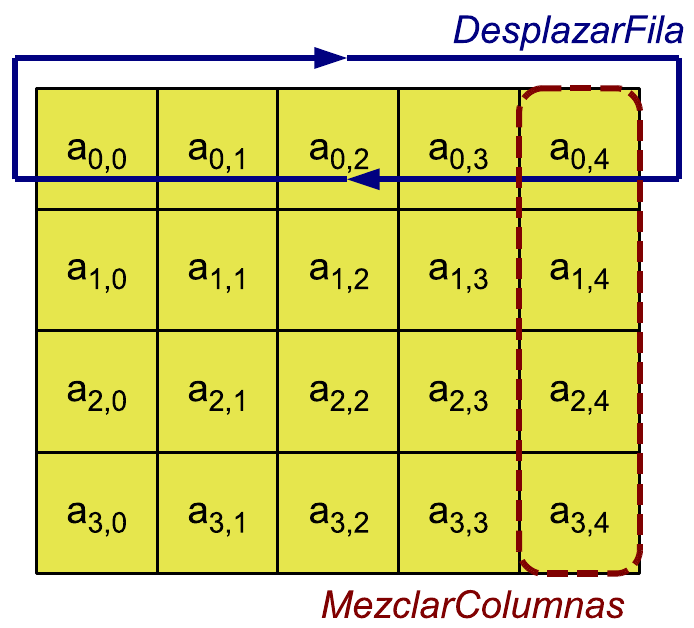
\includegraphics[scale=0.4]{imagenes/aesdesplazarmezclar.png} 
			\caption{Esquema de las funciones $MezclarColumnas$ y $DesplazarFila$ \cite{En2011}}
			\label{desplazarymezclar}
		\end{figure}
%\newpage
	\item \textbf{MezclarColumnas}\\
		Durante la aplicación de esta función se considera cada columna del vector de estado se considera un polinomio cuyos coeficientes pertenecen a $\operatorname{GF}(2^8)$ y se multiplica módulo $x^4+1$ por: $c(x)=03x^3+01x^2+01x+02$ donde 03 es el valor hexadecimal que se obtiene concatenado los coeficientes binarios del polinomio correspondiente en $\operatorname{GF}(2^8)$, en este caso sería 00000011 y por tanto $x+1$ análogamente se haría con los demás.\\
		La inversa de $MezclarColumnas$ se obtiene multiplicando cada columna de la matriz de estado por el polinomio: $d(x)=0Bx^3+0Dx^2+09x+0E$.

\end{description}

\subsection{Cálculo de las Subclaves}
Las subclaves $K_i$ se obtienen de la clave principal $K$ mediante el uso de dos funciones: una de expansión y otra de selección. Siendo $n$ el número de rondas que se van a aplicar, la función de expansión obtiene a partir del valor de $K$ una secuencia de $4(n+1)N_b$ bytes.\\
La función de selección toma consecutivamente de la secuencia obtenida bloques del mismo tamaño que la matriz de estado y los asigna a cada $K_i$.\\

Sea $K(i)$ un vector de bytes de tamaño $4N_k$ conteniendo la clave y sea $W(i)$ un vector de $N_b(n+1)$ registros de 4 bytes, siendo $n$ el número de rondas. 
La función de expansión tiene dos versiones según el valor de $N_k$:

\begin{itemize}
	\item Si $N_k<=6$:
	\begin{algorithm}
		Para $i$ desde 0 hasta $N_{k}-1$ hacer:
		\begin{description}
			$W(i)\leftarrow(K(4·i), K(4·i+1), K(4·i+2), K(4·i+3))$
		\end{description}
		Para $i$ desde $N_k$ hasta $N_{b}·(n+1)$ hacer:\\
			\hspace*{20}$tmp\leftarrow W(i-1)$\\
			\hspace*{20}Si $i$ $mod N_k = 0$\\
			\hspace*{40}$tmp\leftarrow Sub(Rot(tmp))\oplus Rc(i/N_k)$\\
			\hspace*{20}$W(i)\leftarrow W(i-N_k)\oplus tmp$
	\end{algorithm}

	\item Si $N_k>6$:
	\begin{algorithm}
		Para $i$ desde 0 hasta $N_{k}-1$ hacer:
		\begin{description}
			$W(i)\leftarrow(K(4·i), K(4·i+1), K(4·i+2), K(4·i+3))$
		\end{description}
		Para $i$ desde $N_k$ hasta $N_{b}·(n+1)$ hacer:\\
			\hspace*{20}$tmp\leftarrow W(i-1)$\\
			\hspace*{20}Si $i$ $mod N_k = 0$\\
			\hspace*{40}$tmp\leftarrow Sub(Rot(tmp))\oplus Rc(i/N_k)$\\
			\hspace*{20}Si $i$ $mod N_k = 4$\\
			\hspace*{40}$tmp\leftarrow Sub(tmp)$\\
			\hspace*{20}$W(i)\leftarrow W(i-N_k)\oplus tmp$
	\end{algorithm}
\end{itemize}

La función \emph{Sub} devuelve el resultado de aplicar la s-caja de AES a cada uno de los bytes del registro de cuatro que se le pasa como parámetro, la función \emph{Rot} desplaza a la izquierda los bytes del registro y \emph{Rc(j)} es una constante que se define como:
\begin{itemize}
	\item $Rc(j)=(R(j),0,0,0)$.
	\item Cada $R(i)$ es el elemento de $\operatorname{GF}(2^8)$ correspondiente al valor $x^{i-1}$ módulo $x^8+x^4+x^3+x+1$.
\end{itemize}

\section{Criptosistema de Rivest-Shamir-Adleman, RSA}
En esta sección hablaré sobre el cifrado RSA y su funcionamiento, cifrado que como AES, está muy extendido y es utilizado por muchas aplicaciones para cifrar y validar los mensajes.\\
RSA es llamado así en honor a sus creadores Ron Rivest, Adi Shamir y Loenard Adleman, fué desarrollado en 1977. Cabe a destacar que en 1973 se desarrolló en secreto un criptosistema similar por Clifford Cocks para la \emph{Government Communications Headquarters}, que es la agencia de inteligencia de señales británica, y fue desclasificado en 1997\cite{cliffordCocks}.\\
Este criptosistema está basado en el \emph{Teorema de Euler} y en particular en la \emph{Proposición 2.2}.\\

\begin{teorema}
	(Teorema pequeño de Fermat) Sea $a \in \mathbb{Z}$ y $p$ un número primo tal que $mcd(a,p)=1$. Entonces
	$$
		a^{p-1} \equiv 1 \mod p.
	$$
\end{teorema}\vspace*{-10mm}
\begin{proof}
		Sea $a \in \mathbb{Z}$. Tomamos los $p-1$ primeros múltiplos positivos de $a$ que serán de la forma $a, 2a,\dots,(p-1)a$. El resto resultante de dividir los $p-1$ múltiplos positivos de $a$ por $p$ corresponden a 1,2,3,$\dots,p-1$.\\
	Multiplicando ahora todas las congruencias obtenemos 
	$$
		a^{p-1}·(p-1)! \equiv (p-1)! \mod p.
	$$
	Como tenemos que $p\nmid (p-1)!$ se cumple que $mcd(p,p-1)=1$ y por tanto cancelando en la expresión anterior obtenemos
	$$
		a^{p-1} \equiv 1 \mod p.
	$$
\end{proof}

\begin{teorema}
	(Teorema de Euler) Sean a,n $\in \mathbb{Z}$ primos relativos entre sí, entonces $a^{\phi(n)}\equiv 1 \mod n$.
\end{teorema}\vspace*{-10mm}
\begin{proof}
		Sea $n\in \mathbb{Z^+}$ que verifica que $mcd(a,n)=1$ y definimos $S$ como el conjunto de las unidades modulo $n$, $S=\{u_1,u_2,\dots,u_{\phi(n)}\}$ donde $1\leq u_i\leq n-1$, $mcd(u_i,n)=1$ y $u_i\neq u_j$ $\forall i,j \in \{1,\dots,\phi(n)\}$ con $ i\neq j$.\\
	Multiplicando  los elementos de $S$ por $a$ obtenemos 
	$$
		aS=\{au_1,au_2,\dots,au_{\phi(n)}\}
	$$
	Como $mcd(a,n)=1$ entonces $a\mod n$ es una unidad y por tanto $aS$ será el conjunto de las unidades módulo $n$. Y dado que los elementos de $S$ y los de $aS$ coinciden módulo $n$, el producto de estos será el mismo módulo $n$ por lo que obtenemos 
	$$
		u_1u_2\dots u_{\phi(n)} \equiv (au_1)(au_2)\dots (au_{\phi(n)})\mod n.
	$$
	Sacando como factor común $a$ tenemos 
	$$
		u_1u_2\dots u_{\phi(n)} \equiv a^{\phi(n)}u_1u_2\dots u_{\phi(n)}\mod n.
	$$
\end{proof}\\
Donde $\phi(n)$ es la \emph{funclón de Euler} definida como $\phi(n)=|\mathbb{Z}^*_n|$ y se puede calcular de la siguiente forma $$\phi(n)=n\prod_{p_i|n}\left(1-\frac{1}{p_i}\right).$$

\begin{teorema}
		(Teorema Chino del Resto) Sean $a_i\in \mathbb{Z}$ y $p,q \in \mathbb{N}$ tales que $mcd(p,q)$ con $i = 1,2$. Entonces el sistema
		$$
			x\equiv a_1 \mod p,
		$$\vspace*{-10mm}

		$$
			x\equiv a_2 \mod q,
		$$

	tiene solución única módulo $n=pq$. Además, la solución está dada por
	$$
		x\equiv a_1\cdot c_1\cdot d_1 +a_2\cdot c_2\cdot d_2 \mod n,
	$$
	donde se cumple
	$$
		c_1=\frac{n}{p},
	$$
	$$
		c_2=\frac{n}{q},
	$$
		y
	$$
		c_1\cdot d_1 \equiv 1 \mod p,
	$$
	$$
		c_2\cdot d_2 \equiv 1 \mod q.
	$$
	
\end{teorema}

\begin{proposicion}
	Sea $n = pq$, donde p y q son dos primos distintos. Si $x\equiv 1 \mod \phi(n)$, entonces $a^x\equiv a\mod n$ para todo $ a \n \in \mathbb{Z}$.
\end{proposicion}\vspace*{-10mm}
	\begin{proof}
		Si $a$ es múltiplo de $n$, entonces se cumple que $a^x \equiv 0 \equiv a \mod n$. Si $a$ y $n$ son coprimos, $mcm(a,n) = 1$. Entonces tendríamos que $a^x \equiv a \mod n$ por el Teorema de Euler.\\
		Nos quedaría ver ocurre en el caso de $a$ sea múltiplo de $p$ o de $q$, pero no de ambos. Por simetría supondremos que a es múltiplo de $p$, pero no de $q$. En este caso tenemos que $a^x \equiv 0 \equiv a \mod p$  y $a^x \equiv a \mod q$ por el Teorema de Fermat. Como $p$ y $q$ son coprimos entre sí, aplicando el Teorema Chino del Resto se deduce que $a^x \equiv a \mod n$.
	\end{proof}

\subsection{Descripción de RSA}
El contenido de esta sección se basa en \cite{angelRiosMateos}. El funcionamiento de RSA es el siguiente.\\
El usuario elige dos números primos distintos \emph{p} y \emph{q} de buen tamaño ya que mientras más grandes sean más seguro será el cifrado.
Se calcula $n = pq$ y por tanto tenemos que $\phi(n) = (p-1)(q-1)$. A continuación se elige un elemento $c$ coprimo con $\phi(n)$ y se calcula el inverso $d = c^{-1}\mod \phi(n)$. La clave pública será $k=(n,c)$ y la clave privada $k'=(n,d)$.\\
En un principio se consideraba que un tamaño de $n$ de 1024 bits era lo suficientemente grande para que fuera seguro, pero en 2003 Tromer y Shamir mostraron que es posible factorizar números de 1024 bits \cite{1024RSA} por lo que en la actualidad se considera 2048 bits como un tamaño seguro.\\
El conjunto de los mensajes sin cifrar es $\mathcal{M}$, el de los mensajes cifrados será $\mathcal{C}$ y se verifica que $\mathcal{M} = \mathcal{C} = \mathbb{Z}_n$. Las funciones de cifrado y descifrado son respectivamente:
\begin{align*}
	E_{k}:\mathcal{M}\rightarrow\mathcal{C},\\
	a \rightarrow a^c,
\end{align*}
\begin{align*}
	D_{k'}:\mathcal{C}\rightarrow\mathcal{M},\\
	a \rightarrow a^d.
\end{align*}

\subsection{Ataques}
Como hemos visto anteriormente RSA puede ser vulnerable en función de los números primos que se elijan y el tamaño de estos. En este apartado veremos algunos posibles ataques que se podrían llevar a cabo \cite{apuntesCriptografia}.
	\subsubsection{Ataque por módulo común.}
	Este ataque se da cuando hay una mala elección de las claves, típicamente cuando se tienen que generar múltiples claves para varios usuarios y para optimizar, se utiliza el mismo módulo $n$ para todos. Mientras el exponente sea distinto, la clave sigue siendo segura, pero si se da que se cifra el mismo mensaje con los distintos exponentes pero el mismo módulo, se puede descifrar el mensaje original.\\
	Supongamos que tenemos dos claves públicas con el mismo módulo, $(n, e_1)$ y $(n, e_2)$ y además ser verifica que  $mcm(e_1,e_2)$. Supongamos que $re_1+se_2=1$ con $r$\textless $0$\textless $s$. Como se ha visto el mensaje cifrado respectivamente será:
	\begin{align*}
		c_1 = m^{e_1} \mod n\\
		c_2 = m^{e_2} \mod n
	\end{align*}
	Si $(c_1,n) \neq 1$, podemos factorizar $n$ y romper la clave, por lo que podemos suponer que $c_1 \in \mathcal{U}(\mathbb{Z}_n)$. Calculamos $c_1^{-1}$ con el algoritmo extendido de Euclídes tenemos que:
	\begin{align*}
			(c^{-1})^{-r}c_2^s \equiv (m^{e_1})^r(m^{e_2})^s \equiv m^{e_1r+e_2s} = m \mod n.
	\end{align*}

	\subsubsection{Ataque por exponente pequeño.}
	Este ataque se puede hacer cuando se elige un exponente muy pequeño y se cifra el mismo mensaje con distinto módulo. En este caso se puede recuperar el mensaje principal aplicando el Teorema Chino del Resto. Supongamos a varios receptores con claves públicas $(n_i, e)$, con $1\leq i \leq r$, tal que mcd$(n_i, n_j) = 1$ si $i\neq j$ ya que en caso contrario, se podría factorizar el módulo correspondiente mediante el cálculo del MCD.\\
	Llamamos $c_i = m^e \mod n_i$ para cada $1\leq i \leq r$. Seleccionamos $\{i_1,...,i_e \}\subseteq \{1,...,r\}$ y empleando el inverso del isomorfismo de anillos
	\begin{align*}
		\chi:\mathbb{Z}_{n_{i_1}\dots n_{i_e}}\rightarrow \mathbb{Z}_{n_{i_1}}\times \dots \times \mathbb{Z}_{n_{i_e}}
	\end{align*}
	obtenido gracias al Teorema Chino del Resto, se puede calcular
	\begin{align*}
		\chi^{-1}(c_{i_1},\dots,c_{i_e}) = m^e \mod n_{i_1},\dots,n_{i_e}
	\end{align*}
	Dado $m^e$\textless $n_{i_1}\dots n_{i_e}$, se puede obtener $m$ calculando la raíz $e$-ésima en $\mathbb{Z} \subseteq \mathbb{R}$, siempre y cuando $e$ no sea muy grande.

	\subsubsection{Ataque con primos muy próximos.}
	Este ataque se da cuando se eligen dos primos muy próximos entre sí. Dado $n=pq$, con $p$\textless $q$, tenemos que  
	\begin{align*}
			n=\left (\frac{p+q}{2}\right )^2-\left (\frac{p-q}{2}\right )^2.
	\end{align*}
	Si $p$ y $q$ son cercanos, $s=\frac{p-q}{2}$ es pequeño y $t=\frac{p+q}{2}$ es un entero ligeramente mayor que $\sqrt{n}$ tal que $t^2 - n^2$ es un cuadrado perfecto. Probando sucesivamente con valores mayores que $\sqrt{n}$ hasta encontrar una descomposición $n=t^2-s^2$, tenemos que $p=t+s$ y $q=t-s$.

\subsection{Firma digital RSA}
La firma digital con RSA, es una herramienta muy utilizada en las aplicaciones de mensajería para garantizar el no repudio de los mensajes.
Dados dos interlocutores A y B cada uno con sus claves públicas:
\begin{itemize}
	\item para A tenemos $n_A$, $d_A$ y $e_A$,  
	\item para B tenemos $n_B$, $d_B$ y $e_B$.  
\end{itemize}
Para que B sepa que un mensaje \emph{m} ha sido enviado por A se siguen los siguientes pasos:
\begin{enumerate}
	\item A cifra el mensaje \emph{m} usando su clave secreta:
		$$
			S=D_A(m)=m^{d_A} \mod n_A.
		$$
	\item A continuación encripta el mensaje firmado con la clave pública de B:
		$$
			C_B(S)=S\mod n_B.
		$$
		y se lo envía a B.
	\item B recibe $C_B(S)=S^{e_B}$ y lo desencripta: 
		$$
			D_B(S^{e_B})=S \mod n_B.
		$$
	\item Una vez desencriptado la primera parte, B desencripta S con la clave pública de A:
		$$
			C_A(S)=C_A(D_A(m))=(m^{d_A})^{e_A}=m^{d_Ae_B}=m^{1+k\phi(n_A)}\equiv m \mod n_A.
		$$
\end{enumerate}
Una vez hecho esto, B podría afirmar casi con total seguridad que el mensaje ha sido enviado por A garantizando el no repudio del mensaje.

\section{El Problema del Logaritmo Discreto. Diffie-Hellman}
El intercambio de claves \emph{Diffie-Hellman} es un método basado en el Problema del Logaritmo Discreto muy utilizado en las aplicaciones de mensajería al iniciar una conexión. La información de este apartado sobre el logaritmo ha sido obtenida de \cite{angelRiosMateos} y la de \emph{Diffie-Hellman} ha sido obtenida de \cite{En2011}.\\
El Problema del Logaritmo Discreto es definido de la siguiente forma:
\begin{definicion}
	Sea S un semigrupo finito. El Problema del Logaritmo Discreto en el semigrupo S es el de resolver ecuaciones del tipo\\
		$$
			a^x\!=b\;(x\in \mathbb{N}).
		$$
	donde a y b son dos elementos dados de S.
\end{definicion}

La complejidad del Problema del Logaritmo Discreto depende en gran medida del semigrupo $S$ que se elija.
Dado que si se eligiera como $S$ el grupo aditivo $\mathbb{Z}_n$ la solución se obtendría fácilmente resolviendo una ecuación de congruencias del tipo $aX \equiv b \mod n$ que equivaldría a resolver la ecuación diofántica $aX + nY = b$. Pero si ahora $S$ pasara a ser los semigrupos multiplicativos $\mathbb{Z}_n$ o $\mathbb{F}_q$ o sus grupos de unidades, el problema aumentaría su complejidad de manera significativa.\\
Tenemos que $a^x = b$ tiene solución si y solamente si $b$ está en el semigrupo cíclico generado por $a$. Luego si $a$ es un elemento de orden finito de un grupo, se podría suponer en la práctica que $S$ es un grupo cíclico y por ello existiría un isomorfismo con ($\mathbb{Z}_n$, $+$). Luego la dificultad del problema no estaría en la estructura del grupo, sino en reconocer los elementos como potencias de enteros.\\
Se cree que el problema de logaritmo discreto es $\mathbb{NP}$-completo, pero esta conjetura todavía no ha sido demostrada por lo que se considera un problema $\mathbb{NP}$-Intermedio, estos problemas son llamados así porque no están dentro de los problemas $\mathbb{P}$ ni en los problemas $\mathbb{NP}$-completo por ahora \cite{NP-intermedio}.\\
Una vez visto el problema de logaritmo discreto, se explicará el intercambio de claves \emph{Diffie-Hellman}.
\subsection{Intercambio de claves Diffie-Hellman}
Antes de explicar el intercambio de claves \emph{Diffie-Hellman} se introducirá el problema de Diffie-Hellman ya que es la base de este.\\

\begin{definicion}
	Dado el conjunto $\mathbb{Z}^*_{p'}$ con p primo, diremos que $\alpha \in \mathbb{Z}^*_p$ es un generador de $\mathbb{Z}^*_{p'}$ si se cumple:\\
	$$
		\forall b \in \mathbb{Z}^*_{p'},\: \exists i\: tal \: que \: \alpha^i = b
	$$
\end{definicion}

\begin{definicion}
	(El Problema Diffie-Hellman)\\ Dado un número primo p, un número $\alpha$ que sea un \emph{generador} de $\mathbb{Z}^*_{p'}$, $\alpha^a$ y $\alpha^b$, encontrar $\alpha^{ab} \mod p$.  
\end{definicion}

\subsubsection{Intercambio de claves \emph{Diffie-Hellman}}
El intercambio de claves \emph{Diffie-Hellman} es un algoritmo asimétrico basado en el problema de \emph{Diffie-Hellman}, empleado para acordar una clave común en un canal inseguro. Los pasos que se siguen son:\\
Sean $A$ y $B$ dos interlocutores que quieren compartir un valor $K$. Para ello se calcula un número primo $p$ y un generador \alpha de $\mathbb{Z}^*_{p'}$ con $2\leq \alpha \leq p-2$. Esta información es pública y conocida por ambos.
\begin{enumerate}
	\item $A$ escoge un número aleatorio $x$, comprendido entre 1 y $p-2$ y envía a $B$ el valor 
		$$
			\alpha^x \mod p
		$$
	\item Análogamente $B$ escoge un número aleatorio $y$, comprendido entre 1 y $p-2$ y envía a $A$ el valor 
		$$
			\alpha^y \mod p
		$$

	\item $B$ recoge $\alpha^x$ y calcula $K=(\alpha^x)^y \mod p$
	\item $A$ recoge $\alpha^y$ y calcula $K=(\alpha^y)^x \mod p$
\end{enumerate}
Puesto que $x$ e $y$ son conocidos solamente por $A$ y $B$ respectivamente, tenemos que al final solamente $A$ y $B$ acaban conociendo el valor de $K$.\\
A continuación se introducirá la teoría de curvas Elípticas ya que nos permitirá redefinir el intercambio de claves usando estas, generando un problema mucho más complejo y con mayor seguridad el cual es el que se utiliza en aplicaciones de mensajería como \textbf{WhatsApp} y \textbf{Telegram}.

\section{Curvas Elípticas en Criptografía}
La criptografía en curvas Elípticas es considerada como uno de los campos de las matemáticas con más futuro en la criptografía asimétrica.
Esto es debido a sus propiedades que dan lugar a problemas de una gran complejidad computacional análogos a los que presenta la aritmética modular. 
Esto permite que sean utilizadas en algunos algoritmos asimétricos como puede ser el intercambio de claves \emph{Diffie-Hellman} que se verá más adelante. A priori su 
estructura algebraica es más compleja que la de la aritmética modular sin embargo, al implementarlas suelen ser más eficientes y además, con claves más cortas alcanzan 
el mismo nivel de seguridad.\\
El uso de curvas elípticas en criptografía se presentó por primera vez en 1985 por Neal Koblitz y Víctor Miller de manera independiente.\\
La información para esta sección se ha obtenido de \cite{En2011}.

\subsection{Curvas Elípticas en $\mathbb{R}$}
\begin{definicion}
	Una curva definida en $\mathbb{R}$ es el conjunto de puntos del plano (x,y) que cumplen la siguiente ecuación:
$$
	y^2=x^3+ax+b
$$
Donde los coeficientes a,b $\in \mathbb{R}$ defininen de manera unívoca a la curva.
\end{definicion}
Algunas curvas en $\mathbb{R}$ son:

\begin{figure}[H]
	\centering
	\subfloat[\centering Curva $y^2=x^3-4x+1$]{{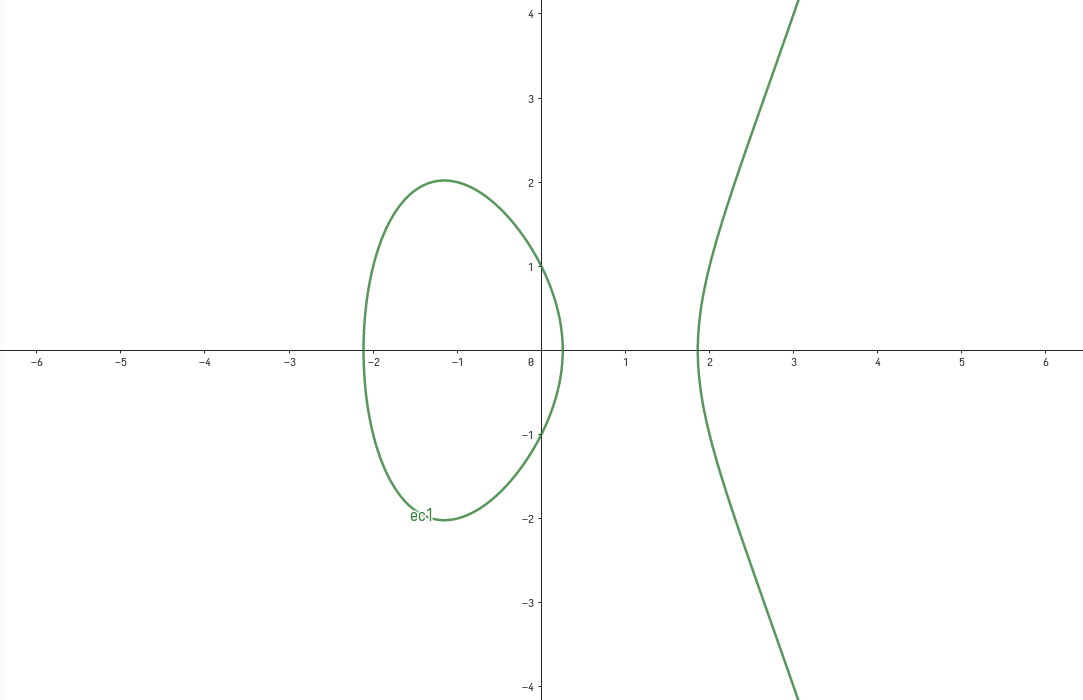
\includegraphics[width=5.9cm]{imagenes/ec1:y^2x^3-4x+1.png}}}
	\qquad
	\subfloat[\centering Curva $y^2=x^3-3x+4$]{{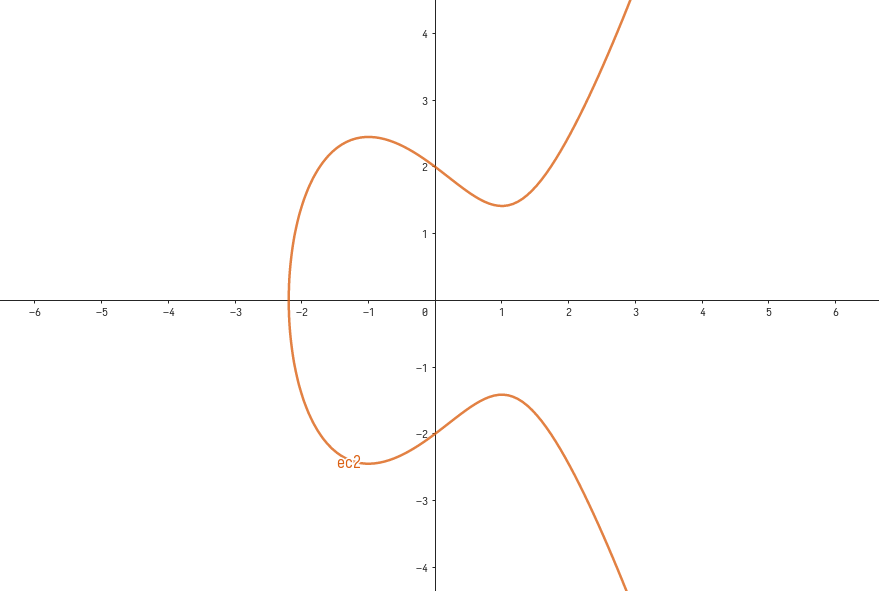
\includegraphics[width=5.9cm]{imagenes/ec2:y^2x^3-3x+4.png}}}
\end{figure}

Si se verifica que $x^3+ax+b$ no tiene raíces múltiples, tendremos que la curva junto con 
el punto $\mathcal{O}$ llamado \emph{punto en el infinito} y la operación $+$ que se definirá 
a continuación es lo que se denomina el \emph{grupo de curva elíptica E(\mathbb{R})}.\\
El punto $\mathcal{O}$ es un punto imaginario situado a una distancia infinita que no tendrá ningún valor en particular.\\

\textbf{Operación $+$ en $\mathbb{R}$}\\
Definido el conjunto en el que se trabajará, definiremos una ley de composición interna $+$.\\
Sean los puntos $r=(r_x,r_y)$, $s=(s_x,s_y)$, $p=(p_x,p_y)$, $t=(t_x,t_y)$ con $r,s,p,t \in E(\mathbb{R})$ la operación $+$ se define como sigue:
\begin{itemize}
	\item $r+\mathcal{O} = \mathcal{O}+r=r,\:\: \forall r \in E(\mathbb{R})$ .
	\item Si $r_x = s_x$ y $r_y = -s_y$, entonces $r=-s$ y además $r+s=s+r=\mathcal{O}$.
	\item Si $r\neq s$ y $r\neq -s$, $r+s=p$ donde $p$ será el opuesto del punto que corta la recta que une $r$ y $t$ con la curva.
	\item Para sumar un punto $p$ con sigo mismo si $p_y\neq0$ se usa la tangente de la curva en $p$. Luego tendremos que $t=p+p$ sera el opuesto de ese punto. Si $p_y=0$ entonces la tangente de la curva será perpendicular al eje de abcisas, por lo que se podría considerar que corta la curva en el infinito, luego $p+p=\mathcal{O}$.
	\item Para sumar $n$ veces un punto $p$ tenemos que si $p_y\neq 0$ entonces sumar $n$ veces $p$ será equivalente a multiplicar $p$ por el escalar $n$ y se representará como $np$. Si $p_y=0$ entonces la suma será:
\end{itemize}
\begin{aligned*}
	\center
	&$2r = r + r = \mathcal{O}$\\
	&$3r = 2r + r = \mathcal{O} + r = r$\\
	&$4r = 3r + r = r + r = \mathcal{O}$\\
	&...\\
\end{aligned}
La suma de curvas elípticas de manera algebraica se define de la siguiente forma:\\
Dados $r=(r_x,r_y)$ y $s=(s_x,s_y)$, tal que $r\noeq-s$, tenemos que $r+s=t$ donde $d=\frac{r_y-s_y}{r_x-s_x},\; t_x=d^2-r_x-s_x,\; t_y=-r_y+d(r_x-t_x)$.
De manera gráfica quedaría de la siguiente manera:\\
\begin{figure}[H]
	\centering
	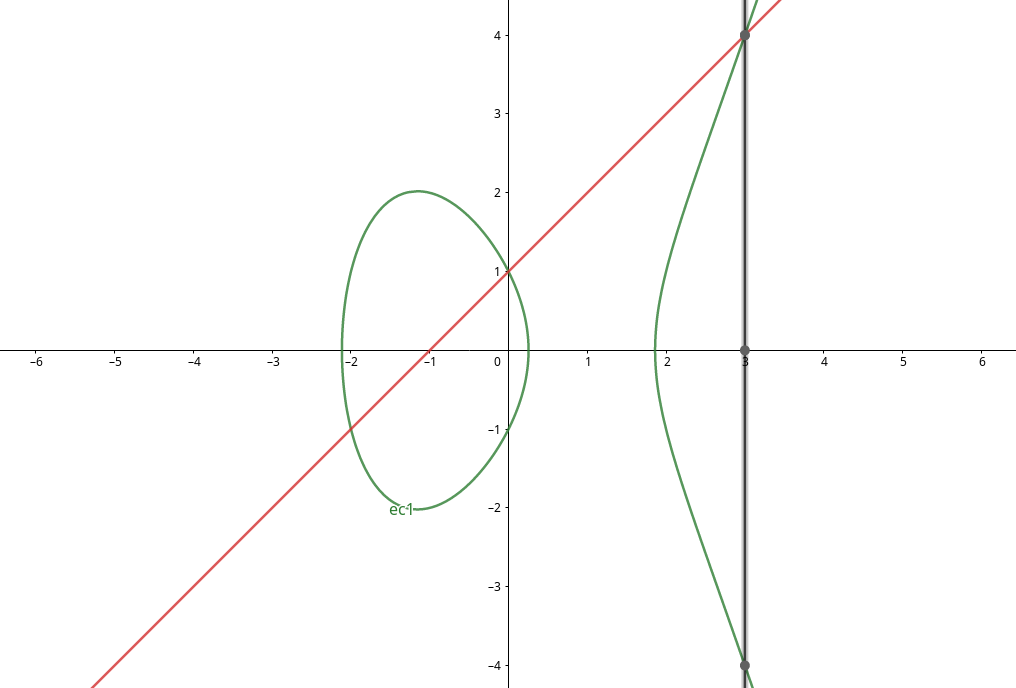
\includegraphics[scale=0.4]{imagenes/sumaCurva.png} 
	\caption{Suma en la curva $y^2=x^3-4x+1$ con $r=(-2,-1),\: s=(0,1),\: -t=(3,4)\: y \: t=(3,-4)$ }
	\label{esquemaecb}
\end{figure}

Una vez definidas las curvas elípticas en $\mathbb{R}$ definiremos las curvas en los cuerpos de Galois $\operatorname{GF}(n)$ y $\operatorname{GF}(2^n)$ cuyo uso esta muy extendido en la criptografía para redefinir el problema de logaritmo discreto.

\subsection{Curvas Elípticas en $\operatorname{GF}(n)$}
Un cuerpo de Galois $\operatorname{GF}(n)$ es el grupo finito generado por un número primo $n$. En este conjunto todos los elementos tienen un inverso, menos el cero por lo que están permitidas las operaciones de suma, resta, multiplicación y división.\\
De manera natural se define el conjunto $E(\operatorname{GF}(n))$ como los puntos $(x,y)$ que verifican la siguiente ecuación: 
$$
	y^2\equiv x^3+ax+b \mod n
$$
Donde al igual que en $E(\mathbb{R})$, $a,b\in{1..n}$ definen de manera unívoca una curva elíptica.\\

%\newpage
\subsubsection{Operación $+$ en $\operatorname{GF}(n)$}
Sean los puntos $r=(r_x,r_y),\: s=(s_x,s_y),\: p=(p_x,p_y),\: t=(t_x,t_y)\in E(\operatorname{GF}(n))$, definimos la operación $+$  como sigue:
\begin{itemize}
	\item $r+\mathcal{O}=\mathcal{O}+r=r,\: \forall r \in \operatorname{GF}(n)$.
	\item Si $r_x=s_x$ y $r_y=s_x+s_y$, entoces se dice que $r$ es el opuesto de $s$, se nota como $r=-s$ y se verifica que $r+s=s+r=\mathcal{O}$.
	\item Si $r\neq s$ y $r\neq-s$, $t=r+s$ se calcula como $d=\frac{s_y-r_y}{s_x-r_x}\mod n,\; t_x=d^2-r_x-s_x \mod n,\; t_y=-r_y+d(r_x-t_x) \mod n$
	\item Si $p_x = 0$ entonces $2p = \mathcal{O}$
\end{itemize}

\subsection{Curvas Elípticas en $\operatorname{GF}(2^n)$}

De manera análoga a $E(\operatorname{GF}(n))$ definimos el conjunto $E(\operatorname{GF}(2^n))$ con la diferencia debida a la estructura de $\operatorname{GF}(2^n)$, la ecuación de curva elíptica es diferente.\\
Dado un polinomio irreducible $p(x)$ de grado $n$, las curvas elípticas se definen como los puntos $(x,y)$ que cumplen la ecuación:
$$
	y^2+xy \equiv x^3+ax^2+b \mod (p(x))
$$
y para que se genere un grupo se tiene que verificar que $b\neq 0$.
Los puntos de una curva serán pares de polinomios de grado $n-1$ y como hemos visto en el apartado anterior, podrán ser representados como cadenas de bits.\\

\subsubsection{Operación $+$ en $E(\operatorname{GF}(2^n))$}
Sean los puntos $r=(r_x,r_y),\: s=(s_x,s_y),\: p=(p_x,p_y),\: t=(t_x,t_y)\in E(\operatorname{GF}(n))$, definimos la operación $+$  como sigue:
\begin{itemize}
	\item $r+\mathcal{O}=\mathcal{O}+r=r,\; \forall r \in E(\operatorname{GF}(2^n))$
	\item Si $r_x=s_x$ y $r_y=s_x+s_y$, entoces se dice que $r$ es el opuesto de $s$, se nota como $r=-s$ y se verifica que $r+s=s+r=\mathcal{O}$.
	\item Si $r\neq s$ y $r\neq-s$, $t=r+s$ se calcula como $d=\frac{s_y-r_y}{s_x-r_x},\; t_x=d^2+d+r_x+s_x+a,\; t_y=d(r_x+t_x)+t_x+r_y$.
	\item Para $t=2p$ con $p_x\neq 0$ se calcula como $d=p_x+\frac{p_y}{p_x}, \: t_x=d^2+d+a, \: t_y=p_x^2+(d+1)t_x$.
	\item Si $p_x=0$ tenemos que $2p=\mathcal{O}$
\end{itemize}

\section{El problema del logaritmo discreto usando curvas elípticas. \emph{Diffie-Hellman}}
En esta sección se hablará sobre el análogo del problema del logaritmo discreto en curvas elípticas y como resultado un análogo del intercambio de claves \emph{Diffie-Hellman}.

\subsection{El problema del logaritmo discreto en curvas elípticas}
Para todo punto $p$ definido en una curva elíptica, se define $\langle p\rangle$ al conjunto $\{\mathcal{O}, p, 2p, ... \}$.
En $E(\operatorname{GF}(n))$ y $E(\operatorname{GF}(2^n))$ los conjutos como los que se han definido, tienen que ser finitos ya que los puntos de las curvas son finitos. Luego para todo punto $q\in \langle p\rangle$ tiene que existir un númer $k \in \mathbb{Z}$ que verifique que $kp=q$.\\
Por lo tanto, el problema del logaritmo discreto en curvas elípticas consiste en hallar dicho número $k$ a partir de $p$ y $q$.
\subsection{Intercambio de claves \emph{Diffie-Hellman} en curvas elípticas}
Una vez visto el problema del logaritmo discreto en curvas elípticas, se explicará el intercambio de claves $Diffie-Hellman$ usando curvas elípticas. Para ello se explicará previamente la conjetura \emph{Diffie-Hellman}. La información de este apartado la he obtenido de \cite{apuntesCriptografia}.\\
Fijamos una curva elíptica $E=E(a,b)$ tal que $|E|=hn$ con $n$ primo y $h$ pequeño. Se fija también $q$ un elemento de orden $n$.
\begin{definicion}
	(Conjetura Diffie-Hellman). Conocidos $p_a=aq$ y $p_b=bq$ para ciertos $1\leq a,\: b\leq n$, calcular $abq$ es equivalente a nivel computacional a calcular $a=\log_q(p_a)$ o $b=\log_q(p_b)$.
\end{definicion}
El protocolo de intercambio de claves queda como:\\

Dadas dos personas A y B que quieren realizar un intercambio de claves.
\begin{itemize}
	\item A y B se ponen de acuerdo en la curva elíptica $E$ y el punto $q\in E$.
	\item A elige aleatoriamente un número $a\in(2,...,n-1)$ y le envía a B $p_a=aq$.
	\item B elige aleatoriamente un número $b\in(2,...,n-1)$ y le envía a A $p_b=bq$.
	\item A calcula $a(p_b)$.
	\item B calcula $b(p_a)$.
	\item La clave compartida es $(ab)q=a(p_b)=b(p_a)$
\end{itemize}

\section{Funciones Hash}
Una función resumen o función hash es un proceso en el cual se transforma un conjunto arbitrario de datos en una nueva serie de caracteres con una longitud fija independiente del tamaño de los datos de entrada, la información para esta sección la he obtenido \cite{aepd}.\\
Las propiedades esperadas de una función hash son:
\begin{itemize}
	\item Se tiene que poder utilizar en contenido digital de cualquier tamaño y formato.
	\item Independientemente del tamaño de la entrada y del tipo, se produce una salida numérica de tamaño fijo.
	\item Para el mismo conjunto de datos de entrada, el resultado siempre es el mismo.
	\item Reconstruir el mensaje original a partir del generado tiene que ser muy complejo, idealmente imposible.
	\item Una variación mínima del mensaje original tiene que producir un hash totalmente distinto, esta propiedad se denomina \emph{difusión}.
	\item Dado un mensaje, tiene que ser muy difícil encontrar otro mensaje con la misma imagen que este \emph{colisión débil}.
	\item Tiene que ser muy costoso encontrar dos mensajes que tengan la misma imagen, esta propiedad es denominada \emph{colisión fuerte}.
	\item Dado un posible valor del espacio imagen, tiene que ser igual de probable que salga este u otro cualquiera. Es decir todos los valores tienen la misma probabilidad de salir.
\end{itemize}

Visto esto, en general, una función hash funciona de la siguiente forma:
\begin{enumerate}
	\item El mensaje de entrada se divide en bloques.
	\item Una fórmula calcula el hash, un valor con un tamaño fijo, para el primer bloque.
	\item Se calcula el hash del siguiente bloque y se suma con el hash calculado previamente.
	\item Se repite de manera análoga con el resto de bloques hasta que se recorren todos.
\end{enumerate}
Las hash que explicaré serán: \emph{MD5, SHA-0} y \emph{SHA-1} que son las funciones antecesoras de la función \emph{SHA-256} que es la que se utiliza mayoritariamente en las funciones de mensajería en la actualidad. Algunas también pueden utilizar SHA-1\\

\subsection{MD5}
MD5 fue diseñada en 1992 por Ron Rivest como una mejora de la función MD4. Es una de las funciones más usadas hasta la fecha aunque su uso esta disminuyendo debido a que se han encontrado algunas debilidades en esta. Uno de los motivos por los que es tan importante es que sirvió como base para desarrollar las funciones SHA-0, SHA-1 y la familia de funciones SHA-2.
La información ha sido obtenida de \cite{Wang2005}.\\
En MD5 el mensaje inicial se fragmenta en bloques de 512 bits y la salida es un hash de 128 bits, el proceso de generación de este es el siguiente:

\begin{enumerate}
	\item El mensaje se rellena con un único bit '1' seguido de 0-511 bits '0'. A continuación se añade una representación de 64 bits de la longitud del mensaje donde el número de ceros es elegido para asegurar que la longitud total del mensaje es un múltiplo de 512 bits. El mensaje se divide en bloques de 512 bits: $M_1,...,M_n$.
	\item Para la primera iteración se utiliza un buffer predefinido:
	$$
		h_0=(67452301_x, EFCDAB89_x, 98BADCFE_x, 10325476_x, C3D2E1F0_x).
	$$
	\item Cada bloque $M_j$ es pasado por la función de compresión junto con el valor actual de $h_{j-1}$, la salida es el nuevo valor de $h_j$, la operación se puede resumir en:
	$$
		h_j=compresión(M_{j-1},h_{j-1}).
	$$
	\item $h_n$ es la salida de la función hash.
\end{enumerate}
Donde la función hash funciona de la siguiente manera:
\begin{enumerate}
	\item Se divide el bloque $M_j$ de 512 bits en bloques 16 bloques de 32 bits $m_0,m_1,...,m_{15}$. 
\item Divide $h_{j-1}$ en 4 registros \emph{A, B, C} y \emph{D} como:
	$$
		h_{j-1} = (A_0, B_0, C_0, D_0, E_0).
	$$
	\item Para $i=0,...,63$ hacemos:
	$$
		A_{i+1}=B_i+((A_i+\Phi_i(B_i,C_i,D_i)+W_i+T_i)\lll S_i),
	$$
	$$
		D_{i+1}=A_{i+1}+((D_i+\Phi_{i+1}(A_{i+1},B_i,C_i)+W_{i+1}+T_{i+1})\lll S_{i+1}),
	$$
	$$
		C_{i+1}=D_{i+1}+((C_i+\Phi_{i+2}(D_{i+1},A_{i+1},B_i)+W_{i+2}+T_{i+2})\lll S_{i+2}),
	$$
	$$
		B_{i+1}=C_{i+1}+((B_i+\Phi_{i+3}(C_{i+1},D_{i+1},A_{i+1})+W_{i+3}+T_{i+3})\lll S_{i+3}).
	$$
	Donde la operación $+$ es la operación ADD $\mod 32$, $T_{i+j}$ y $S_{i+j}\; (j=0,1,2,3)$ son constantes dependientes de la iteración y $W_i$ son palabras del mensaje.\\
	En cada ronda se utiliza una función $\Phi_i(X,Y,Z)$ que depende de la iteración:
	\begin{description}
		\item $\Phi_i(X,Y,Z)=(X\wedge Y)\vee (\overline{X}\wedge Z),\; 0\leq i\leq 15,$
		\item $\Phi_i(X,Y,Z)=(X\wedge Z)\vee (Y\wedge \overline{Z}),\; 16\leq i\leq 31,$
		\item $\Phi_i(X,Y,Z)=X\oplus Y\oplus Z,\; 32\leq i\leq 47,$
		\item $\Phi_i(X,Y,Z)=Y\oplus (X\vee \overline(Z)),\; 48\leq i\leq 63$
	\end{description}
\end{enumerate}
En la imagen siguiente se puede ver un esquema del proceso de generación del hash usando MD5.
\begin{figure}[htb]
	\centering
	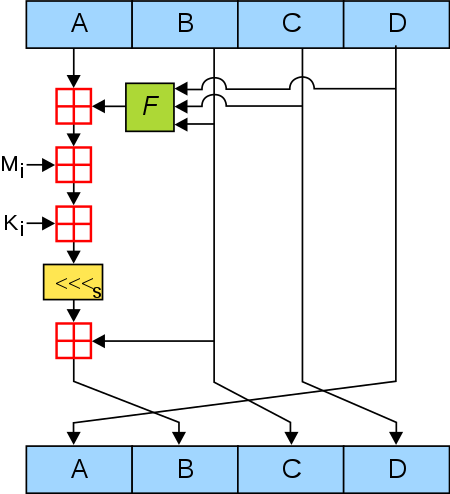
\includegraphics[scale=0.5]{imagenes/md5.png} 
	\caption{Esquema de los pasos seguidos en MD5 \cite{fotosmd5}.}
\end{figure}

\subsection{SHA-0}
SHA-0 es una función hash que apareció publicado en el Federal Information Processing Standard (FIPS-180) por el NIST en 1993 \cite{Penard2008}. Está basado en \emph{MD4} y \emph{MD5}. El algoritmo transforma un mensaje de cualquier tamaño hasta $2^{64}$ bits y los transforma en hashes de 160 bits.\\
El funcionamiento de SHA-0 es el siguiente \cite{sha0}:
\begin{enumerate}
	\item Al igual que en MD5, el mensaje se rellena con un único bit '1' seguido de 0-511 bits '0'. A continuación se añade una representación de 64 bits de la longitud del mensaje donde el número de ceros es elegido para asegurar que la longitud total del mensaje es un múltiplo de 512 bits. El mensaje se divide en bloques de 512 bits: $M_1,...,M_n$.
	\item Para la primera iteración se utiliza un buffer predefinido:
	$$
		h_0=(67452301_x, EFCDAB89_x, 98BADCFE_x, 10325476_x, C3D2E1F0_x).
	$$
	\item Cada bloque $M_j$ es pasado por la función de compresión junto con el valor actual de $h_{j-1}$, la salida es el nuevo valor de $h_j$, la operación se puede resumir en:
	$$
		h_j=compresión(M_j,h_{j-1}).
	$$
	\item $h_n$ es la salida de la función hash.
\end{enumerate}
Los pasos seguidos en la función de compresión son:
\begin{enumerate}
	\item Se divide el bloque $M_j$ de 512 bits en bloques 16 bloques de 32 bits $W_0,W_1,...,W_{15}$. 
	\item Se expanden los 16 bloques de 32 bits en 80 bloques a partir de la siguiente ecuación en recurrencias:
	$$
		W_i=W_{i-3}\oplus W_{i-8}\oplus W_{i-14}\oplus W_{i-16},\; i=16,...,79.
	$$
	Esta expansión se nota como exp(.).
	\item Divide $h_{j-1}$ en 5 registros \emph{A, B, C, D} y \emph{E} como:
	$$
		h_{j-1} = (A_0, B_0, C_0, D_0, E_0).
	$$
	\item Para $i=0,...,79$ hacemos:
	$$
		A_{i+1}=(A_i\lll5)+f_i(B_i,C_i,D_i)+E_i+K_i) \mod 2^{32},
	$$
	$$
		B_{i+1}=A_i,\: C_{i+1}=(B_i\lll30),\: D_{i+1}=C_i,\: E_{i+1}=D_i.
	$$
	Donde las funciones y las constantes están definidas en la tabla \ref{tablasha0}.
	\item La salida de la función sería:
	$$
		h_n=(A_0+A_{80}, B_0+B_{80}, C_0+C_{80}, D_0+D_{80}, E_0+E_{80}).
	$$
\end{enumerate}

\begin{table}[H]
	\begin{center}
		\begin{tabular}{| l | l | l |}
				\hline
				Rondas & $f_i(B,C,D)$ & $K_i$\\ \hline
				$0\leq i\leq 19$ & $BC\vee BD$ & $5AD9EBA1_x$\\ \hline
				$20\leq i\leq 39$ & $B\oplus C\oplus D$ & $6ED9EBA1_x$\\ \hline
				$40\leq i\leq 59$ & $BC\vee BD\vee CD$ & $8F1BBCDC_x$\\ \hline
				$60\leq i\leq 79$ & $B\oplus C\oplus D$ & $CA62C1D6_x$\\ \hline
		\end{tabular}
		\caption{Funciones y constantes usadas en la función de compresión de SHA-0 \cite{sha0}.}
	\label{tablasha0}
	\end{center}
\end{table}

\subsection{SHA-1}
La función SHA-1 es una función hash diseñada en 1995 por la \emph{National Security Agency} (NSA) dado que que se encontró varias colisiones y vulnerabilidades en la función SHA-0 \cite{Penard2008}.\\
Su funcionamiento es muy similar al de la función SHA-0 variando en las funciones y variables usadas en las distintas rondas de la función de compresión. En la tabla \ref{tablasha1} se pueden ver los nuevos valores utilizados.\\
\begin{table}[htb]
	\begin{center}
		\begin{tabular}{| l | l | l |}
				\hline
				Rondas & $f_i(B,C,D)$ & $K_i$\\ \hline
				$0\leq i\leq 19$ & $(B\wedge C)\oplus (\overline{B}\wedge D)$ & $5A827999_x$\\ \hline
				$20\leq i\leq 39$ & $B\oplus C\oplus D$ & $6ED6EBA1_x$\\ \hline
				$40\leq i\leq 59$ & $(B\wedge C)\oplus (B\wedge D) \oplus (C\wedge D)$ & $8FABBCDC_x$\\ \hline
				$60\leq i\leq 79$ & $B\oplus C\oplus D$ & $CA62C1D6_x$\\ \hline
		\end{tabular}
		\caption{Funciones y constantes usadas en la función de compresión de SHA-1 \cite{sha1}.}
		\label{tablasha1}
	\end{center}
\end{table}

En siguiente imagen se puede observar un esquema del proceso para obtener un el hash seguido por las funciones  SHA-0 y SHA-1 donde \textbf{F} será la función de compresión.
\begin{figure}[htb]
	\centering
	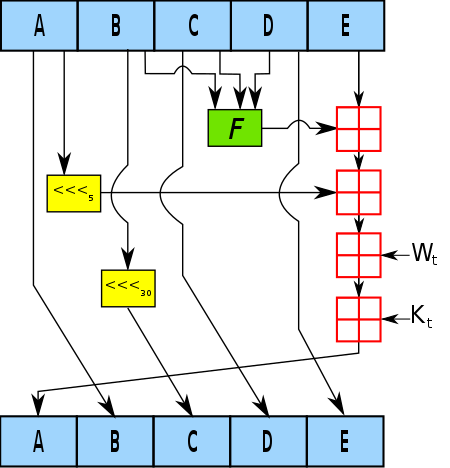
\includegraphics[scale=0.5]{imagenes/sha0-1.png} 
	\caption{Esquema de los pasos seguidos en SHA-0 y SHA-1 \cite{fotosha10}.}
\end{figure}

\subsection{SHA-256}
La función SHA-256 pertenece a la familia SHA-2 que es un conjunto de funciones hash diseñadas por la NSA en 2001 \cite{Penard2008}. Esta familia está compuesta por las funciones SHA-224, SHA-256, SHA-384 y SHA-512 donde el número del final indica el tamaño de bloque en el que se dividirá el mensaje. Nos centraremos en la función SHA-256 que como he comentado anteriormente es la que se utiliza en las aplicaciones de mensajería actualmente.\\
El funcionamiento de las función es el siguiente\cite{Function2016}:\\
\begin{enumerate}
	\item Al igual que en SHA-0 y SHA-1 se rellena el mensaje de la misma manera y se fragmenta en bloques de 512 bits: $M_1,...,M_n$.
	\item Para la primera iteración se utiliza un buffer predefinido:
	$$
		h_0=(H_1, H_2, H_3, H_4, H_5, H_6, H_7, H_8),
	$$
	donde:\\
	$H_1=6A09E776$\\
	$H_2=BB67AE85$\\
	$H_3=3C6EF372$\\
	$H_4=A54FF53A$\\
	$H_5=510E527F$\\
	$H_6=9B05688C$\\
	$H_7=1F83D9AB$\\
	$H_8=5BE0CD19$\\
	\item Cada bloque $M_j$ es pasado por la función de compresión junto con el valor actual de $h_{j-1}$, la salida es el nuevo valor de $h_j$, la operación se puede resumir en:
	$$
		h_j=compresión(M_j,h_{j-1}).
	$$
	\item $h_n$ es la salida de la función hash.
\end{enumerate}
Los pasos seguidos en la función de compresión son:
\begin{enumerate}
	\item Se divide el bloque $M_j$ de 512 bits en bloques 16 bloques de 32 bits $W_0,W_1,...,W_{15}$. 
	\item Se expanden los 16 bloques de 32 bits en 63 bloques a partir de la siguiente ecuación en recurrencias:
	$$
		W_i=\sigma_1(W_{j-2})+W_{j-7}+\sigma_0(W_{j-16}),\; i \in \{16...63\}.
	$$
	\item Divide $h_{j-1}$ en \emph{A, B, C, D, E, F, G} y \emph{H} como:
	$$
		h_{j-1} = (A_0, B_0, C_0, D_0, E_0, F_0, G_0, H_0).
	$$
	\item Para $i=0,...,63$ hacemos:
	$$
		A_{i+1}=H_i+\Sigma_1(E_i)+Ch(E_i,F_i,G_i)+K_j+W_j+\Sigma_0(A_i)+Maj(A_i,B_i,C_i),
	$$
	$$
		B_{i+1}=A_i,\: C_{i+1}=B_i,\: D_{i+1}=C_i,\: F_{i+1}=E_i\: G_{i+1}=F_i,\: H_{i+1}=G_i,
	$$
	$$
		E_{i+1}=D_i+H_i+\Sigma_1(E_i)+Ch(E_i,F_i,G_i)+K_j+W_j.
	$$
	Donde las funciones y las constantes están definidas en la tabla \ref{tablasha0}.
	\item La salida de la función sería:
	$$
		h_j=(A_0+A_{63}, B_0+B_{63}, C_0+C_{63}, D_0+D_{63}, E_0+E_{63}, F_0+F_{63}, G_0+G_{63}, H_0+H_{63}).
	$$
\end{enumerate}
Donde tenemos que:
$$
	Ch(x,y,z) = (x\wedge y)\oplus (\overline{x}\wedge z),
$$
$$
	Maj(x,y,z) = (x\wedge y)\oplus (x\wedge z)\oplus (y\wedge z),
$$
$$
	\Sigma_0(x) = (x\ggg2)\oplus (x\ggg13)\oplus (x\ggg22),
$$
$$
	\Sigma_1(x) = (x\ggg6)\oplus (x\ggg11)\oplus (x\ggg25),
$$
$$
	\sigma_0(x) = (x\ggg7)\oplus (x\ggg18)\oplus (x\lll3),
$$
$$
	\sigma_1(x) = (x\ggg17)\oplus (x\ggg19)\oplus (x\lll10).
$$

%\newpage
En la siguiente imagen podemos ver un esquema de los pasos seguidos en las funciones SHA-2.\\
\begin{figure}[htb]
	\centering
	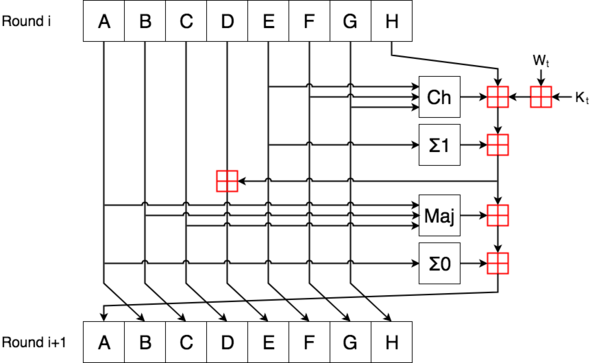
\includegraphics[scale=0.5]{imagenes/sha2.png} 
	\caption{Esquema de los pasos seguidos en las funciones de la familia SHA-2 \cite{sha2wikipedia}.}
\end{figure}

Con esto concluye el capítulo en el cual se han introducido todas las herramientas necesarias para entender los criptosistemas de las aplicaciones de mensajería. En el próximo capítulo procederé a explicar los criptosistemas utilizados en algunas de las aplicaciones de mensajería más populares.

%
\chapter{Aplicaciones de Mensajería}

Los cifrados que se van a desarrollar serán los de Telegram, Whatsapp Facebook Chat y Signal, y AppleChat.

\section{Telegram (MTProto)}
MTProto es el protocolo de datos con el Telegram cifra sus mensajes. Fue desarrollado por el matemático Nikolái Dúrov y financiado por Pável Dúrov. Al contrario que la mayoría de cifrados, MTProto esta enfocado en ser multisesión e independiente de la plataforma y el transporte de archivos independiente de su formato. MTProto tiene dos versiones:
\begin{itemize}
	\item \textbf{MTProto v1:} En esta versión los mensajes son cifrados con el algoritmo \emph{SHA-1} y en 2017 fue reemplazado ya que se encontró una vulnerabilidad en la intercepción de mensajes debido a \emph{SHA-1}.
	\item \textbf{MTProto v2:} En 2017 se actualizó MTProto, en esta versión se cambió el cifrado \emph{SHA-1} por \emph{SHA-256} que es el que se utiliza actualmente y el que se desarrollará a continuación.
\end{itemize}
Referencias: \cite{Miculan2021} \cite{WebProto}

\subsection{Descripción general y resumen de los componentes}
MTProto 2.0 es una suite de protocolos criptográficos diseñados para implementar de manera rápida, escalable y segura intercambio de mensajes sin depositar esa responsabilidad en la seguridad del transporte debajo de dicho protocolo.
El protocolo esta subdividido en tres componentes virtuales independientes:
\begin{itemize}
	\item \textbf{Componente de alto nivel:} Define el método por el cual las consultas de la API y las respuestas se convierten en mensajes binarios. 
	\item \textbf{Capa criptográfica(autorización):} Define el método por el cual los mensajes están cifrados antes de ser enviados a través del protocolo de transporte.
	\item \textbf{Componente de transporte:} Define el método por el cual el cliente y el servidor para transmitir los mensajes sobre otro protocolo de red como HTTP, HTTPS, WS, WSS, TCP o UDP.
\end{itemize}
Y se pueden resumir en:
\begin{description}
	\item \textbf{Componentes de alto nivel(Lenguajes de consulta/API RPC):}
Desde el punto de vista del componente de alto nivel, el cliente y el servidor intercambian mensajes dentro de una sesión.\\
La sesión se adjunta al cliente en lugar de una conexión \emph{websocket/http/https/tcp.} 
Además, cada sesión tiene asociada a clave ID de usuario mediante la cual se logra la autorización.\\ 
Pueden estar abiertas varias conexiones a un servidor, los mensajes pueden ser enviados en cualquier dirección a través de cualquiera de las conexiones.
Cuando se usa el protocolo UDP, una respuesta puede ser devuelta por una dirección de IP distinta.\\
Hay diferentes tipos de mensajes:
\begin{itemize}
		\item \textbf{LLamadas RPC(cliente-servidor):} LLamadas a los métodos de la API.
		\item \textbf{Respuestas RPC(servidor-cliente):} Resultados de las llamadas RPC.
		\item \textbf{Notificación del estado de los mensajes}
		\item \textbf{Consultas de estado de mensaje}
		\item \textbf{Mensaje multiparte o contenedor}
\end{itemize}
Desde el punto de vista de protocolos de bajo nivel, un mensaje es un flujo de datos alineados con 4 o 16 bytes de límite.
Los primeros campos en un mensaje están fijos y son usados por el sistema criptográfico o de autorización.\\
Cada mensaje, consiste en un \emph{Message Identifier} de 64 bits, \emph{número de secuencia del mensaje dentro de una sesión}, \emph{longitud} de 32 bits y \emph{cuerpo del mensaje} de cualquier tamaño siempre y cuando sea múltiplo de 4. 
Además cuando un contenedor o un mensaje simple se envían, una \emph{cabecera interna} se añade al principio del mensaje, luego el mensaje es cifrado y se le añade una \emph{cabecera externa} la cual será una \emph{clave de identificación} de 64 bits y una \emph{clave del mensaje} de 128 bits.\\
El \emph{cuerpo} del mensaje normalmente consiste en un \emph{tipo mensaje} de 32 bits seguido de los \emph{parámetros dependientes del tipo}.\\
Los números están escritos en \emph{little endian}. Sin embargo los números muy grandes(2048 bits) usados en \textbf{RSA} y \textbf{DH} están escritos en \emph{big endian} porque es lo que hace la biblioteca \textbf{OpenSSL}.
	\item \textbf{Autorización y Cifrado:}
			Antes de que un mensaje sea transmitido por la red usando un protocolo de transporte, este es cifrado añadiendo una cabecera externa la cual es insertada al principio del mensaje y contiene:
	\begin{itemize}
		\item \emph{Key Identifier} de 64 bits
		\item \emph{Message Key} de 128 bits
	\end{itemize}
Una clave de usuario junto con una clave de mensaje definen una clave de 256 bits la cual es la que cifra el mensaje usando un cifrado \emph{AES-256}.
La primera parte del mensaje cifrado contiene datos variables(sesión, id del mensaje, número de secuencia) los cuales influyen en la clave del mensaje. La clave del mensaje es definida como los 128 bits iniciales del mensaje cifrado con \emph{SHA-256}, 
además los mensajes en varias partes están cifrados como un solo mensaje.\\
Lo primero que tiene que hacer la aplicación cliente es crear una clave de autorización que se genera normalmente la primera vez que se ejecuta la aplicación y por lo general nunca cambia.\\
Para prevenir potenciales ataques debido a la apropiación de la clave de autorización MTProto soporta \emph{Perfect Forward Secrecy} tanto en los chats en la nube como en los chats secretos.
	\item \textbf{Sincronización de la hora:}
Si la hora de un cliente difiere de la hora del servidor, el servidor podría empezar a ignorar los mensajes de este y recíprocamente el cliente a los mensajes del servidor debido a que el mensaje tenga un indentificador inválido del mensaje.\\
Bajo estas circunstancias, el servidor enviará un mensaje especial al cliente el cual contendrá la hora correcta, este mensaje será el primero en el caso de que también se envíe un grupo de mensajes.\\
Habiendo recibido el mensaje, el cliente primero ejecutará una sincronización de la hora y después verificará la \emph{Message Key} para ver si es correcto.\\
En caso de que no sea correcto, el cliente deberá generar una nueva sesión para asegurar la monotonía de los \emph{Message Keys}.
\end{description}

\subsection{Descripción de las claves:}
En esta sección se describirán las distintas claves que entran en juego en el proceso de cifrado y descifrado de MTProto 2.0 \cite{telegram2}.

\begin{description}
	\item \textbf{Authorization Key (auth\textunderscore key)}\\
	Es una clave de 2048 bit compartida por el dispositivo del cliente y el servidor, se crea durante el registro del usuario, se almacena en el dispositivo de este mediante el protocolo de intercambio de claves \emph{Diffie-Hellman} y nunca se transmite a través de la red. Cada \emph{Authorization key} es única y dependiente del usuario, aunque un usuario puede tener más de una ya que Telegram permite tener sesiones persistentes en diferentes dispositivos. En caso de ser necesario estas claves pueden ser bloqueadas para siempre como por ejemplo podría pasar si un dispositivo con sesión persistente se pierde.

	\item \textbf{Server Key}\\
	Es una clave RSA de 2048 bits usada por el servidor para firmar sus mensajes durante el proceso de registro y la clave se está generando. La aplicación tiene una clave publica del servidor que puede ser utilizada para verificar la firmas pero no para firmar mensajes. La clave privada del servidor es almacenada en este y raramente cambia.

	\item \textbf{Key Identifier (auth\textunderscore key\textunderscore id)}\\
	Se usan los 64 bits menos significativos del hash \emph{SHA1} de la \emph{Authorization Key} para indicar que clave en particular se ha usado para cifrar el mensaje. Las claves tienen que ser identificadas unívocamente y en caso de colisión, la \emph{Authorization Key} se regenera. Un identificador Zero Key significa que el cifrado no se usa y esto está permitido para muy pocos mensajes usados durante el registro para generar la clave en el intercambio \emph{Diffie-Hellman}.
	
	\item \textbf{Session}\\
	Es un número de 64 bits generado aleatoriamente por el cliente para distinguir entre sesiones individuales como pueden ser diferentes instancias de la aplicación creadas con la misma \emph{Authorization Key} donde una instancia de la aplicación es la conjunción de la \emph{Key Identifier} y la \emph{Session}.\\
	Bajo ninguna circunstancia un mensaje perteneciente a una sesión puede ser enviado a otra.

	\item  \textbf{Server Salt}\\
	Es un número de 64 bits generado aleatoriamente que cambia cada 30 minutos independiente de las sesiones por una petición del servidor. Una vez generado el nuevo salt todos los mensajes tienen que tenerlo aunque se aceptan los mensajes con el salt previo. Es necesario para proteger ante ciertos ataques como podría ser ajustar el reloj de la víctima en un momento futuro.

	\item \textbf{Message Identifier (msg\textunderscore id)}\\
	Es un número de 64 bits dependiente del tiempo usado únicamente para identificar mensajes sin sesión. Los \emph{Message Identifiers} son divisibles por 4, los \emph{Message Identifiers} del servidor módulo 4 dan 1 si el mensaje es una respuesta a un mensaje del cliente y dan 3 en otro caso. 
	Los \emph{Message Identifiers} del cliente deben incrementarse monótonamente, igualmente con los del servidor y tienen que ser aproximadamente igual a $unixtime*2^{32}$, donde \emph{unixtime} es un sistema para la descripción de instantes de tiempo definida como la cantidad de segundos transcurridos desde la medianoche UTC del 1 de enero de 1970. 
	De esta manera, el \emph{Message Identifier} señala el momento aproximado en el que el mensaje fue creado siendo rechazado alrededor de 300 segundos después o 30 segundos antes de ser creado (necesario como medida de protección de ataques de repetición).  

	\item \textbf{Content-related Message}\\
	Un mensaje requiere un reconocimiento explícito. Esto incluye todos los mensajes de usuario y muchos de servicio, a excepción de contenedores y otros reconocimientos.

	\item \textbf{Message Sequence Number (msg\textunderscore seqno)}\\
	Un número de 32 bit igual o el doble del número de mensajes \emph{content-related} creados por el remitente antes de este mensaje y posteriormente se va incrementado en uno si el mensaje es del tipo \emph{cotent-related}. Cabe a destacar que como un contenedor se genera después de su contenido, su \emph{Message Sequence Number} será siempre igual o mayor a los números de mensajes contenidos en él.

	\item \textbf{Message Key (msg\textunderscore key)}\\
	En el protocolo \textbf{MTProto 2.0}, la \emph{Message Key} se define como los 128 bits del medio del hash \emph{SHA-256} del mensaje que va a ser cifrado antepuesto por un fragmento de 32 bytes de la clave de autorización.\\
	En el protocolo \textbf{MTProto 1.0}, la \emph{Message Key} se definía como los 128 bits menos significativos del hash \emph{SHA-1} del mensaje a ser cifrado, los bytes de relleno eran excluidos en el cálculo del hash. La \emph{Authorization Key} no estaba involucrada en este cálculo.

	\item \textbf{Internal (cryptographic) Header}\\
	Una cabecera de 16 bytes añadida antes de que el mensaje o el contenedor sea cifrado. Consiste en el \emph{Server Salt} de 64 bits y la \emph{Session} de 64 bits.

	\item \textbf{External (cryptographic) Header}\\
	Una cabecera de 24 bytes que se añade antes de que el mensaje o el contenedor sea cifrado. Consiste en la \emph{auth\textunderscore key\textunderscore id} de 64 bits y la \emph{msg\textunderscore key} de 128 bits.

	\item \textbf{Payload}\\
	Es el \emph{External Header} + mensaje cifrado o contenedor.
\end{description}

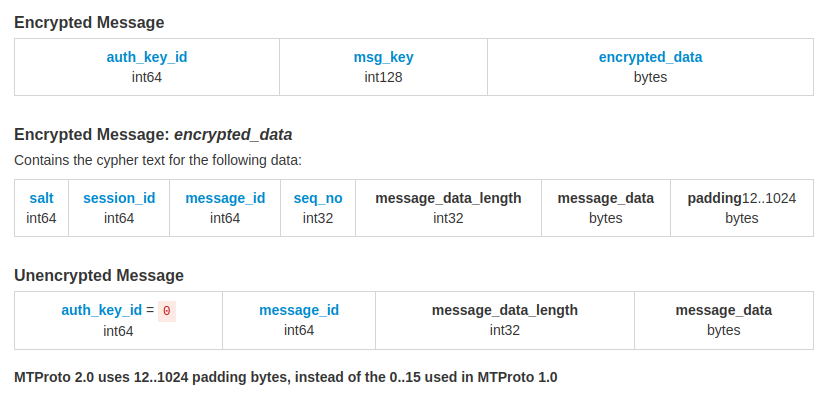
\includegraphics[scale=0.5]{imagenes/MTProto2.png} 

\subsection{Creación de la \emph{Authorization Key}}
Como hemos visto en el apartado anterior la \emph{Authorization Key} se genera durante el registro del usuario en la aplicación. El formato de las consultas usa \emph{Binary Data Serialization} ya que MTProto requiere que los tipos de datos estén en formato binario y \emph{TL Language} que sirve para describir el sistema utilizado de tipos y funciones.\\
Los números de gran tamaño son transmitidos como cadenas que contienen la secuencias de bytes en formato \emph{big endian}, los números de menor tamaño como pueden ser los \emph{int, long int128...} usan normalmente el formato \emph{little endian} aunque si pertenecen al \emph{SHA1} los bytes no son reorganizado.\\
Una vez introducido los formatos que seguirán las consultas y los números veamos los pasos que se siguen en la creación de la \emph{Authorization Key}.

\begin{enumerate}
	\item El cliente envía una consulta al servidor, en esta consulta irá el \emph{nonce} que es un número aleatorio \emph{int128} generado por el cliente que servirá para para que el servidor lo identifique, este número no es secreto y a partir de ese momento irá incorporado en todas las consultas. 
	
	\item El servidor le responde enviándole: 
	\begin{itemize}
		\item \emph{server\textunderscore nonce}: Es un número aleatorio \emph{int128} generado por el servidor que sirve para que el cliente lo identifique y al igual que el \emph{nonce} no será secreto e irá incluido en las siguientes consultas y respuestas. 
		\item \emph{pq}: Es una representación de un número natural en formato \emph{big endian} que es el producto de dos números primos, \emph{pq} por lo general verifica $pq \leq 2^{63}-1$
		\item \emph{server\textunderscore public\textunderscore key\textunderscore fingerprints}: Es una lista de \emph{fingerprints} de claves RSA públicas.
	\end{itemize}

	\item El cliente descompone \emph{pq} en factores primos tal que $p$\textless$q$. Con esto empieza el intercambio de claves Diffie-Hellman.

	\item El cliente envía una nueva consulta que contiene:
	\begin{itemize}
		\item \emph{nonce}
		\item \emph{server\textunderscore nonce}
		\item \emph{p}: Factor obtenido en el paso anterior, es de tipo \emph{long}.
		\item \emph{q}: El otro factor obtenido en el paso anterior, al igual que \emph{p} es de tipo \emph{long}.
		\item \emph{public\textunderscore key\textunderscore fingerprint}: Una de las \emph{fingerprints} obtenida de la lista enviada por el servidor en el paso anterior, es del tipo \emph{long}.
		\item \emph{encrypted\textunderscore data}: Mensaje cifrado obtenido aplicando RSA a \emph{data} y \emph{server\textunderscore public \textunderscore key} donde:
		\begin{itemize}
			\item \emph{data}: Es una serialización de \emph{pq}, \emph{p}, \emph{q}, \emph{nonce}, \emph{server\textunderscore nonce}, \emph{new\textunderscore nonce} (un nuevo número aleatorio generado por el cliente y desde este paso conocido por el cliente y el servidor) y \emph{dc} o una serialización de \emph{pq}, \emph{p}, \emph{q}, \emph{nonce}, \emph{server\textunderscore nonce}, \emph{new\textunderscore nonce}, \emph{dc} y \emph{expires\textunderscore in}.

			\item \emph{dc} es un identificador de la consulta, es del tipo \emph{int}.

			\item \emph{expires\textunderscore in} es el tiempo en el que expira la consulta, es del tipo \emph{int}.
		\end{itemize}
	\end{itemize}
	Después de este paso alguien podría interceptar la consulta y modificarla con una cosulta suya haciendo un ataque \textbf{man-in-the-middle}. 
	Este ataque no sería muy efectivo, ya que el único elemento que podría modificar sería \emph{new\textunderscore nonce} porque los demás están cifrados y el resultado sería que el atacante genere una \emph{Authorization\textunderscore key} propia independiente de la del cliente haciendo que el ataque no sea efectivo.

	\item El servidor responde enviando:
		\begin{itemize}
			\item \emph{nonce}
			\item \emph{server\textunderscore nonce}
			\item \emph{encrypted\textunderscore answer}: Respuesta cifrada que es del tipo \emph{string} y contiene:
			\begin{itemize}
				\item \emph{new\textunderscore nonce\textunderscore hash}: Son los 128 bits menos significativos de \emph{SHA1(new\textunderscore nonce)}.
				\item \emph{answer}: Es una serialización de \emph{nonce}, \emph{server\textunderscore nonce}, \emph{g}, \emph{dh\textunderscore prime}, \emph{g\textunderscore a} y \emph{server\textunderscore time}.
				\item \emph{answer\textunderscore with\textunderscore hash}: Es una generación con la función hash \emph{HASH1} quedando de la siguiente forma: \emph{SHA1(answer)+answer+(0-15 bytes aleatorios)} de manera que la longitud sea divisible por 16, es del tipo \emph{string}.
				\item \emph{answer\textunderscore aes\textunderscore key}: \emph{SHA1(new\textunderscore nonce + server\textunderscore nonce) + substr(SHA1(server\textunderscore nonce + new\textunderscore nonce), 0, 12)} y es del tipo \emph{string}.
				\item \emph{tmp\textunderscore aes\textunderscore iv}: \emph{substr(SHA1(server\textunderscore nonce + new\textunderscore nonce), 12, 8) + SHA1(new\textunderscore nonce + new\textunderscore nonce) + substr(new\textunderscore, 0, 4)}
				\item \emph{encrypted\textunderscore answer}: \emph{AES256\textunderscore ige\textunderscore encrypt(answer\textunderscore with\textunderscore hash, tmp\textunderscore aes\textunderscore key, tmp\textunderscore aes\textunderscore iv)} donde:
				\begin{itemize}
					\item \emph{tmp\textunderscore aes\textunderscore key}: Es una clave de 256 bits
					\item \emph{tmp\textunderscore aes\textunderscore iv}: Es un vector de inicialización de 256 bits.
				\end{itemize}
				Al igual que en el resto de las instancias que usan el cifrado AES, a los datos cifrados se le añaden bytes aleatorios de forma que el tamaño sea divisible por 16.
			\end{itemize}
		\end{itemize}
	Después de este paso \emph{new\textunderscore nonce} sigue siendo únicamente conocido por el cliente y el servidor de esta manera el cliente garantiza que el servidor es el que está al otro lado de la comunicación y que la respuesta de este es correcta, ya que los datos están cifrados usando \emph{new\textunderscore nonce}.\\
	El cliente comprueba que \emph{p} el cual es un primo usado en Diffie-Hellman, es un número primo seguro de 2048 bits, es decir, se tiene que verificar que \emph{p} y $\frac{p-1}{2}$ son primos, además, $2^{2047}$\textless \emph{p} \textless $2^{2048}$, y \emph{g} genera un subgrupo cíclico con orden primo $\frac{p-1}{2}$.\\
	Si la verificación tarda mucho tiempo, cosa que ocurre en dispositivos antiguos, se ejecutarían solo 15 iteraciones en el algoritmo de Miller-Rabin para garantizar que \emph{p} y $\frac{p-1}{2}$ sean primos con una probabilidad de error muy baja, alrededor de una millonésima, y dejar el resto de iteraciones para después, ejecutándose estas de fondo.

	\item El cliente genera un número aleatorio \emph{b} de 2048 bits y lo envía al servidor en un mensaje que contiene:
		\begin{itemize}
			\item \emph{nonce}
			\item \emph{server\textunderscore nonce}
			\item \emph{encrypted\textunderscore data} que se descifra de la siguiente manera:
				\begin{itemize}
					\item \emph{g\textunderscore b} = $g^b$ mod \emph{dh\textunderscore prime}
					\item \emph{data} que es una serialización donde:
						\begin{itemize}
							\item \emph{nonce}
							\item \emph{server\textunderscore nonce}
							\item \emph{retry\textunderscore id} que vale 0 en el primer intento y en caso contrario, vale \emph{auth\textunderscore key\textunderscore aux\textunderscore hash} del intento fallido anterior y es del tipo \emph{long}.
							\item \emph{g\textunderscore b} que es del tipo \emph{string}.
						\end{itemize}
					\item \emph{data\textunderscore with\textunderscore hash} que es: \emph{SHA1(data)+data+(0-15 bytes aleatorios de manera que el tamaño sea divisible por 16)}.
					\item \emph{encrypted\textunderscore data} que es: \emph{AES256\textunderscore ige\textunderscore encrypt(data\textunderscore with\textunderscore hash, tmp\textunderscore aes\textunderscore key, tmp\textunderscore aes\textunderscore iv)}.
				\end{itemize}
		\end{itemize}
	\item Una vez hecho los pasos previos tendríamos que \emph{auth\textunderscore key} vale $g^{ab}$ mod \emph{dh\textunderscore prime}, en el servidor se calcula como \emph{$g\textunderscore b^{a}$ mod \emph{dh\textunderscore prime}} y en el cliente se calcula como $g\textunderscore a^b$ mod \emph{dh\textunderscore prime}.
	\item \emph{auth\textunderscore key\textunderscore hash} se calcula como los 64 bits de menor prioridad de \emph{SHA1(auth\textunderscore key)}. El servidor comprueba si existe alguna otra clave con el mismo \emph{auth\textunderscore hash} y responde de alguna de las siguientes tres formas
	\begin{enumerate}
		\item Una serialización de: 
			\begin{itemize}
				\item \emph{nonce}
				\item \emph{server\textunderscore nonce}
				\item \emph{new\textunderscore nonce\textunderscore hash1}
			\end{itemize}
		\item Una serialización de:
			\begin{itemize}
				\item \emph{nonce}	
				\item \emph{server\textunderscore nonce}
				\item \emph{new\textunderscore nonce\textunderscore hash2}
			\end{itemize}
		\item Una serialización de:
			\begin{itemize}
				\item \emph{nonce}	
				\item \emph{server\textunderscore nonce}
				\item \emph{new\textunderscore nonce\textunderscore hash3}
			\end{itemize}
	\end{enumerate}
	Donde \emph{new\textunderscore nonce\textunderscore hash1}, \emph{new\textunderscore nonce\textunderscore hash2} y \emph{new\textunderscore nonce\textunderscore hash3} son los 128 bits menos significativos de SHA1 de la cadena de bytes obtenida al añadir a \emph{new\textunderscore nonce} un byte con el valor 1,2 o 3 respectivamente y seguido de \emph{auth\textunderscore key\textunderscore hash}.\\
	\emph{Auth\textunderscore key\textunderscore aux\textunderscore hash} son los 64 bits más significativos de \emph{SHA1(auth\textunderscore key)}.
	Si algo falla durante estos pasos, el cliente volvería al paso 6 y generándose un nuevo \emph{b}. Al mismo tiempo se define \emph{server\textunderscore salt} como \emph{substr(new\textunderscore nonce, 0, 8)} XOR \emph{substr(server\textunderscore nonce, 0, 8)}.\\
	
\end{enumerate}
\textbf{Gestión de errores}

Si el cliente no obtiene alguna respuesta del servidor en un intervalo de tiempo determinado se repite la consulta, análogamente ocurre con el servidor. Sin embargo si el servidor no obtiene una segunda respuesta del cliente en 10 minutos, reiniciará la conexión y el cliente tendrá que empezar de nuevo.

\subsection{Generando la clave y el vector de inicialización de AES}
En esta sección hablaré de como se generan la clave de autorización (\emph{auth\textunderscore key}) y de la clave del mensaje (\emph{msg\textunderscore key}) necesarias para calcular la clave de AES (\emph{aes\textunderscore key}) y el vector de inicialización de 256 bits (\emph{iv\textunderscore aes}) usados para cifrar los mensajes en MTProto 2.0.\\
El algoritmo consiste en:
\begin{enumerate}
	\item Calculamos \emph{msg\textunderscore key\textunderscore large} como \emph{SHA256(substr(auth\textunderscore key, 88+x, 32)+plaintext+random\textunderscore padding)}.
	\item Calculamos \emph{msg\textunderscore key} como \emph{substr(msg\textunderscore key\textunderscore large, 8, 16)}.
	\item Calculamos \emph{sha256\textunderscore a} como \emph{SHA256(msg\textunderscore key+substr(auth\textunderscore key, x, 36))}.
	\item Calculamos \emph{sha256\textunderscore b} como \emph{SHA256(substr(auth\textunderscore key, 40+x, 36)+msg\textunderscore key)}
\end{enumerate}
Y una vez hechos estos pasos, ya podemos calcular la clave para AES y el vector de inicialización.
\begin{itemize}
	\item \textbf{\emph{aes\textunderscore key}}: \emph{substr(sha256\textunderscore a, 0, 8)+substr(sha256\textunderscore b, 8, 16)+substr(sha256\textunderscore a, 24, 8)}.
	\item \textbf{\emph{aes\textunderscore iv}}: \emph{substr(sha256\textunderscore b, 0, 8) + substr(sha256\textunderscore a, 8 16)+substr(sha256\textunderscore b, 24, 8)}.
\end{itemize}
\emph{x} vale 0 cuando los mensajes van del cliente al servidor y 8 cuando los mensajes van del servidor al cliente.\\
Los 1024 bits menos significativos de la \emph{auth\textunderscore key} no se utilizan para el cálculo ya que estos se usan para cifrar la copia local de los datos recibidos del servidor además, los 512 bits menos significativos no se almacenan en el servidor por lo que si el cliente pierde la clave o la contraseña del dispositivo, no se podrán descifrar los datos locales. Un esquema del proceso se puede ver en \ref{mtproto2}
\newpage
\begin{figure}[htb]
	\centering
	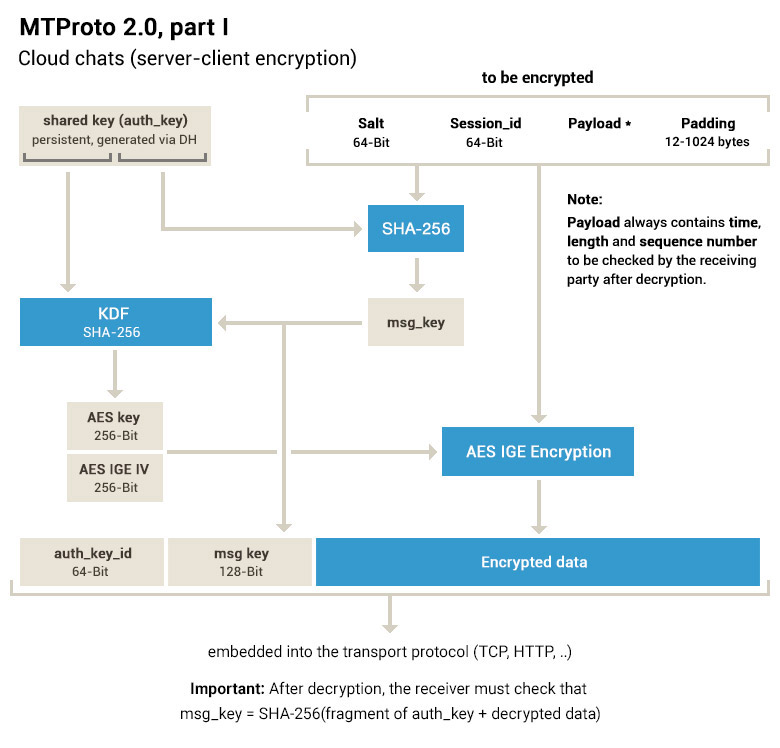
\includegraphics[scale=0.4]{imagenes/diagramaMTProto.jpg} 
	\caption{Esquema del cifrado de mensajes usado en MTProto 2.0}
	\label{mtproto2}
\end{figure}

\subsection{Envío de mensajes}
Una vez realizado el intercambio de claves mediante \emph{Diffie-Hellman} y la generación de la clave y el vector de inicialización de AES ya se podrían enviar mensajes cifrados entre el cliente y el servidor utilizando \emph{AES256}.
Los protocolos de transporte que están disponibles son:
\begin{itemize}
	\item \emph{TCP}
	\item \emph{WebSocket}
	\item \emph{WebSocket} sobre \emph{HTTPS}
	\item \emph{HTTP}
	\item \emph{HTTPS}
	\item \emph{UDP}
\end{itemize}


%
%\input{capitulos/04_Analisis}
%
%\input{capitulos/05_Diseno}
%
%\input{capitulos/06_Implementacion}
%
%\input{capitulos/07_Pruebas}
%
%\input{capitulos/08_Conclusiones}
%
%%\chapter{Conclusiones y Trabajos Futuros}
%
%

%%\nocite{*}

\bibliographystyle{plainurl}
\bibliography{bibliografia/library.bib}\addcontentsline{toc}{chapter}{Bibliografía}
%
%\appendix
%\input{apendices/manual_usuario/manual_usuario}
%%\input{apendices/paper/paper}
%\input{glosario/entradas_glosario}
% \addcontentsline{toc}{chapter}{Glosario}
% \printglossary
%\chapter*{}
%\thispagestyle{empty}

\end{document}
